% JHEP format. The style package jheppub supplies the page layout, natbib, hyperref and the
% \abstract macro; the bibliography style JHEP.bst is selected at the end of this file.
% amsmath, amssymb, graphicx are loaded by jheppub, so they are not loaded again here.
\documentclass[11pt,a4paper]{article}
\usepackage{amsmath,amssymb,latexsym}
\usepackage[svgnames]{xcolor}
\usepackage{jheppub}
\usepackage{braket}
\usepackage{float}
\graphicspath{{figures/}}
\usepackage{bm}
\usepackage{setspace}
%\usepackage{arydshln}% | in matrix
\usepackage{hepunits}
%\usepackage{ulem}
\usepackage{mciteplus}
\usepackage{booktabs,array}
\usepackage{enumitem}



\newcommand{\introrevision}[1]{{\color{red}\hypersetup{citecolor=red}#1}}
\setlength{\emergencystretch}{2em}
\sloppy
\newcommand{\shift}{\qquad~~}
\newcommand{\ep}{\varepsilon}
\newcommand{\nn}{\nonumber}
\newcommand{\nd}{\mathrm{d}}
\newcommand{\spdot}{\!\cdot\!}

\newcommand{\be}{\begin{equation}}
\newcommand{\ee}{\end{equation}}
\newcommand{\ba}{\begin{eqnarray}}
\newcommand{\ea}{\end{eqnarray}}
\newcommand{\dd}{\mathrm d}
\newcommand{\ii}{\mathrm i}
\newcommand{\Id}{\mathbb I}
\newcommand{\diag}{\operatorname{diag}}
\newcommand{\cV}{\mathcal V}
\newcommand{\cE}{\mathcal E}
\newcommand{\cH}{\mathcal H}
\newcommand{\cM}{\mathcal M}
\newcommand{\cB}{\mathcal B}
\newcommand{\cR}{\mathcal R}
\newcommand{\cN}{\mathcal N}
\newcommand{\Emb}{\operatorname{Emb}}
\def\ie{\begin{equation}\begin{aligned}}
\def\fe{\end{aligned}\end{equation}}
\def\ma{\mathcal}
\title{MadStree: a package for quickly evaluating arbitrary tree-level cosmological correlator}
\author{Spongebob Squarepants, Patrick Star}

% JHEP style: the abstract is a macro collected in the preamble and printed by \maketitle,
% which also typesets the table of contents, so no \tableofcontents is written in the body.
\abstract{
\texttt{MadStree} is a Mathematica package to compute arbitrary tree-level cosmological correlators with scalar propagators numerically. It can deal with both massless and massive propagators. In this framework, a given dS tree diagram will be reduced to corresponding master integrals, and these master integrals will be solved by IBP and differential equations numerically. The usage of this package is described in detail via some examples.
}

\begin{document}
\maketitle

\section{Introduction}
\label{sec:introduction}

Tree-level cosmological correlators in de~Sitter (dS) space are the basic objects of
inflationary perturbation theory: after the in-in Feynman rules are applied, a correlator is a sum
of time integrals whose integrands contain Hankel functions for massive propagators, exponentials
for the external energies, and theta functions for the time-ordered propagators\cite{Weinberg:2005vy,Chen:2017ryl}. Lots of analytic methods have been developed, including the cosmological bootstrap \cite{Arkani-Hamed:2018kmz,Baumann:2019oyu,Baumann:2020dch,Pajer:2020wnj,Pajer:2020wxk,Cabass:2021fnw,Baumann:2022jpr,Pimentel:2022fsc,Jazayeri:2022kjy,Qin:2022fbv,Wang:2022eop,Qin:2023ejc,Aoki:2024uyi,Liu:2024str,
Qin:2025xct,Xianyu:2025lbk}, Mellin techniques \cite{Sleight:2019mgd,Sleight:2019hfp,Sleight:2020obc,Sleight:2021plv,Premkumar:2021mlz,Qin:2022lva,Qin:2022fbv,Xianyu:2023ytd,Qin:2024gtr}, spectral decompositions \cite{Marolf:2010zp,Xianyu:2022jwk,Loparco:2023rug,Werth:2024mjg,
Qin:2025xct,Zhang:2025nzd,Altshuler:2025qmk} and dispersive methods \cite{Liu:2024xyi,Das:2026vfv}. See also \cite{Wang:2021qez,Werth:2023pfl,Pinol:2023oux,Werth:2024aui,Chen:2024glu} for some recent numerical studies. 

A systematic
evaluation of such integrals was developed in \cite{Chen:2023iix}, where the
Integration-By-Parts (IBP) relations were generalized from polynomial integrands to the Hankel
integrand case. In \cite{Chen:2024glu} the iterative IBP reduction and the d log-form
differential equations of arbitrary tree-level correlators were given in uniform, closed form, and
the boundary conditions were determined by power series expansions together with blow-up. Once the differential equation and the boundary conditions are known, the master integrals can be solved
numerically at any ordinary point of the kinematic space. As a complement to \cite{Chen:2023iix}, we will show the derivation of these methods for massless internal lines. Compared with the analytic methods, this IBP-based method is faster when we want the numeric value of a large number of points. In addition, since this method is also based on the differential equation, it is easy to do analytic continuation using numeric techniques.

\texttt{MadStree} is a Mathematica package that numerically evaluates arbitrary tree-level
cosmological correlators of scalar fields in de~Sitter space. The evaluation implements the
framework mentioned above. The user input is an arbitrary tree diagram or loop diagram\footnote{For loop diagrams, we do not compute the loop momentum integral.}. \texttt{MadStree}
returns the master-integral values at every requested point, with their status and error
estimates, exportable to CSV/JSON; in the regulator mode it returns the certified lowest power
and the Laurent coefficients of the pole and finite parts. This mode is needed because whenever the vertex time powers take special values, the time integrals are defined only after regularization: the integral can sit on a
pole and the time IBP becomes singular, while the boundary expansion at $\tau\to0$ degenerates
as soon as its branch exponents resonate. Introducing a common analytic regulator $\varepsilon$
on the time powers makes the system generic, and the physical $\varepsilon\to0$ limit is then
taken from the reconstructed Laurent series.

The paper is organized as follows. In Sec.~\ref{sec:method} we derive the formulas
underlying the package. We review the definition of the vertex integral family and the derivation of their IBP relations, differential equations, and boundary conditions. We also discuss the simplification of the massless case in this section, and the reduction of several propagators that share one theta function, whose derivation is collected in App.~\ref{app:theta}. In Sec.~\ref{sec:usage} we describe how to use the package: the loading procedure, the input formats and core functions, the numerical workflow and the reconstruction of the regulator series. We also summarize the principal options and common pitfalls. In Sec.~\ref{sec:examples-section} we collect the examples shipped with the release and present two application examples. We close with a summary and outlook in Sec.~\ref{sec:summary}.

\section{Statement on AI Use}
\label{sec:ai-use}

The notation, the functionality and the public interfaces of this package were designed by the
authors, who also indicated the overall direction and the strategy of the derivation recorded in
Sec.~\ref{sec:method}; the concrete derivation was then worked out by agent programs driven by
large language models. The package was implemented by those same programs on the basis of the
authors' guidance and of the derivation results above; to verify the reliability of the package,
the authors designed the following verification tasks, listed together with the source of the
reference data in each case.

\begin{itemize}
  \item \textbf{Single-vertex families and the massive two-vertex correlator.} The exact
        differential equations, the boundary coefficients and the numerically transported results
        are compared with the known results of \cite{Chen:2024glu}, which are computed by an
        independent multivariate hypergeometric construction.
  \item \textbf{The massive three-vertex tree graph.} The package results are checked against two
        independent sources at once: the output of an agent program that received only the
        previously hand-written two-vertex code and generalized it to three vertices along its own
        route, and the published eight-branch result of \cite{Xianyu:2023ytd}. The agent output was
        itself first checked against that published result before being used as a reference, so the
        package is validated both by independently generated code and by the published numbers.
  \item \textbf{IBP relations and differential equations.} These are compared with the
        \texttt{dSIBP} package \cite{dSIBP:inPreparation}, which is released in the same repository
        as this one, \url{https://github.com/J7C/dSIBP-Packages}. \texttt{dSIBP} samples naive IBP
        seeds and solves the resulting linear reduction system, whereas the present package applies
        the general formulas derived in Sec.~\ref{sec:method} directly and never re-solves an IBP
        system; the agreement therefore tests the closed formulas themselves.
\end{itemize}

\section{IBP reduction and differential equations for tree-level dS integrals}
\label{sec:method}

This section derives the objects the package computes: the integral family of a tree-level dS
correlator, the IBP relations that reduce the family, the d log-form differential equation (DE) of
its master integrals, and the boundary data that fixes the solution. Two references underlie the
construction: \cite{Chen:2023iix} derives the generalized IBP relations and the one-step
lowering/raising recurrences, and \cite{Chen:2024glu} organizes them into a uniform d log-form DE
whose boundary conditions come from the $\tau\to0$ expansion together with blow-up.

Two points distinguish the present section from those references and fix the organization of the
material. First, we work in the prefactor convention that the package implements, in which the
Hankel block carries $z^{+\nu}$ rather than the $z^{-\nu}$ of the printed formulas of
\cite{Chen:2023iix,Chen:2024glu}; relative to those papers this is the single simultaneous
replacement $\nu\to-\nu$ in every occurrence, and after performing it no further translation is
needed anywhere below (Sec.~\ref{sec:notation}). Second, the one and only structural difference
from \cite{Chen:2023iix} is the massless internal line: that reference never uses the extra
reduction relations of a massless bulk propagator to compress the four endpoint states of a
massless \emph{full} propagator into a single two-state factor shared by the whole edge, while the
package does. We therefore build the IBP relations from the start out of the three local building
blocks of Sec.~\ref{sec:ibp} rather than re-deriving the single-vertex family, and we mark every
quantity quoted from \cite{Chen:2023iix} before that extra relation is imposed by a superscript
${\rm unreduced}$ (defined in eq.~\eqref{eq:unreduced-space}). Section~\ref{sec:common-theta} and
App.~\ref{app:theta} treat a further case that \cite{Chen:2023iix} does not discuss: several
propagators that share one and the same theta function.

\subsection{Notation: propagators, the integral family and index conventions}
\label{sec:notation}
\label{sec:conventions}

\paragraph{In-in Feynman rules and asymptotic behavior.}
Cosmological correlators are evaluated in the Schwinger--Keldysh (SK) formalism: the operator
product is ordered along a closed time path, and each vertex is labelled by a contour branch,
written \texttt{"+"} or \texttt{"-"}, with one time integration $\int_{-\infty}^0\dd\tau_v$ per
vertex. With the positive-frequency mode function
\begin{equation}
  u(\tau;k)=-\ii\sqrt{\frac{\pi}{2}}\,
  e^{\ii\pi(\nu/2+1/4)}H_{\rm Hubble}^{(d-1)/2}
  (-\tau)^{d/2}H^{(1)}_\nu(-k\tau),
  \label{eq:mode-function}
\end{equation}
where $k=|\bm k|$ and $\nu^2=d^2/4-m^2/H_{\rm Hubble}^2$ for a minimally coupled scalar in $d$
spatial dimensions ($\nu$ is real or imaginary for $d=3$), the bulk-to-bulk propagators are
\begin{equation}
  G^>(k;\tau_1,\tau_2)\equiv u(\tau_1,k)u^*(\tau_2,k),\qquad
  G^<(k;\tau_1,\tau_2)\equiv u^*(\tau_1,k)u(\tau_2,k),
  \label{eq:bulk-bulk-propagators}
\end{equation}
and the time-ordered combinations used by the in-in rules are
\begin{align}
  G^{++}&=G^>\theta(\tau_1-\tau_2)+G^<\theta(\tau_2-\tau_1),
  &G^{--}&=G^<\theta(\tau_1-\tau_2)+G^>\theta(\tau_2-\tau_1),
  \notag\\
  G^{+-}&=G^<,
  &G^{-+}&=G^>.
  \label{eq:sk-propagators}
\end{align}
Throughout, $\theta_{ij}\equiv\theta(\tau_i-\tau_j)$ denotes the theta function of the time
difference of vertices $i$ and $j$. Bulk-to-boundary propagators of massless fields,
$G^\pm\propto(1\mp\ii k\tau)e^{\pm\ii k\tau}$, enter only as pure-exponential blocks. The Hankel
functions obey
\begin{equation}
  \partial_\tau^2H^{(1,2)}_\nu(-k\tau)
  +\frac1\tau\,\partial_\tau H^{(1,2)}_\nu(-k\tau)
  +\left(k^2-\frac{\nu^2}{\tau^2}\right)H^{(1,2)}_\nu(-k\tau)=0,
  \label{eq:hankel-eom}
\end{equation}
with the two asymptotic regimes
\ie
  &H^{(1)}_\nu(-k\tau)=c_1(-k\tau)^\nu(1+O(\tau^2))+c_2(-k\tau)^{-\nu}(1+O(\tau^2)),
  \quad \tau\to0^-,\\
&c_1=e^{-\ii\pi\nu}c[\nu]\,, \quad c_2=c[-\nu]\,, \quad
c[\nu]\equiv \frac{ 2^{-\nu } \Gamma (-\nu )}{\ii \pi }  \, .
  \label{eq:hankel-tau0}
\fe
and
\begin{align}
  &H^{(1)}_\nu(-k\tau)\sim\sqrt{\frac2\pi}(-k\tau)^{-1/2}
  e^{-\ii k\tau-\ii\pi(\nu/2+1/4)},\notag\\
  &H^{(2)}_\nu(-k\tau)\sim\sqrt{\frac2\pi}(-k\tau)^{-1/2}
  e^{\ii k\tau+\ii\pi(\nu/2+1/4)},
  \quad -k\tau\to\infty.
  \label{eq:hankel-infinity}
\end{align}
The first regime fixes the boundary conditions of the time integrals; the second justifies the
Wick rotation used in the numerical evaluation of Sec.~\ref{sec:numerics}.

\paragraph{The two-state $h$ block.}
A tree-level correlator with $V$ vertices contains one time integration per vertex, and each
integrand is a product of the elementary factors
\begin{equation}
  \left\{e^{\ii k\tau},\;H^{(1,2)}_\nu(-k\tau),\;
  \partial_\tau H^{(1,2)}_\nu(-k\tau),\;\theta(\tau_j-\tau_k)\right\}.
  \label{eq:integrand-factors}
\end{equation}
Following \cite{Chen:2024glu}, the Hankel prefactor and the time derivative are absorbed into two
states of one function system. We use the convention of the package, in which the prefactor is the
\emph{positive} power of $z$,
\begin{equation}
  \begin{aligned}
  h^{(s)}(\nu,0;z)&\equiv z^{+\nu}H^{(s)}_\nu(z),\\
  h^{(s)}(\nu,1;z)&\equiv-\frac1k\,\partial_\tau h^{(s)}(\nu,0;z)=\partial_z h^{(s)}(\nu,0;z),
  \qquad z=-k\tau,
  \end{aligned}
  \label{eq:h-definition}
\end{equation}
with $s\in\{1,2\}$ the Hankel branch. Superscripts on $h$ will always denote the branch, never a
power or a label. The alternative normalization $h(\nu,0;z)=z^{-\nu}H_\nu(z)$ used in
\cite{Chen:2023iix,Chen:2024glu} is related to \eqref{eq:h-definition} by $\nu\to-\nu$, because
$H^{(1)}_{-\nu}=-e^{\ii\pi\nu}H^{(2)}_\nu$ and $H^{(2)}_{-\nu}=-e^{-\ii\pi\nu}H^{(1)}_\nu$
differ only by branch-independent phases; equivalently, with $\nu_{\rm ref}$ the symbol printed in
those two papers, $\nu_{\rm ref}=-\nu$ \emph{everywhere at once} --- in the equation of motion
below, in the Wronskian, in $\text{M}_1$, in the contact powers, in the recurrences and in the
d log potentials. For a heavy field $\nu=\ii\mu$ with real $\mu$ this reduces to
$e^{-\pi\mu}H^{(2)}_{-\ii\mu}(z)=H^{(2)}_{\ii\mu}(z)$, and we shall use exactly this identity in
Sec.~\ref{sec:remaining} to trade the conjugate-order endpoint basis of \cite{Chen:2024glu} for the
common-order basis of the package.

Since the Hankel equation involves $\nu^2$ only, the two normalizations satisfy different
first-order systems but the same second-order one up to $\nu\to-\nu$. In the convention
\eqref{eq:h-definition}, with $\bm h=(h(\nu,0;z),h(\nu,1;z))^T$ and
$P_1\equiv\tfrac12(\Id-\sigma_3)=\diag(0,1)$,
\begin{equation}
  \partial_\tau\bm h
  =\left[-\ii k\sigma_2-\frac{1-2\nu}{\tau}\,P_1\right]\bm h,
  \label{eq:h-first-order-system}
\end{equation}
where $\sigma_{1,2,3}$ are the Pauli matrices and $\Id$ the $2\times2$ identity; the equivalent
dimensionless equation of motion is
\begin{equation}
  \partial_z^2h(\nu,0;z)+\frac{1-2\nu}{z}\,\partial_zh(\nu,0;z)+h(\nu,0;z)=0,
  \label{eq:h-dimensionless-eom}
\end{equation}
whose constant term is $1$; the physical $k^2$ enters only through $\partial_\tau=-k\partial_z$.

\paragraph{The vertex integral family and its index conventions.}
For a vertex carrying $n$ massive legs, the one-vertex family (an $n$-fold Hankel vertex integral
family) reads
\begin{equation}
  f^{(a_0)}_{\tilde{\bm a};\bm s}
  =\int_{-\infty}^0\dd\tau\,(-\tau)^{\nu_0+a_0}e^{\ii p_0\tau}
  \prod_{i=1}^{n}h^{(s_i)}(\nu_i,a_i;-k_i\tau),
  \qquad a_0\in\mathbb Z,\quad a_i,s_i\in\{0,1\},
  \label{eq:vertex-integral-family}
\end{equation}
where the indices have the following meanings, which we reuse for the whole graph:
\begin{itemize}
  \item $\nu_0$ is the power of the vertex time, $s_i\in\{1,2\}$ is the Hankel branch chosen at
        leg $i$ by the SK type of the line that ends there, $a_i\in\{0,1\}$ is the \emph{state bit}
        --- the index of the two components of \eqref{eq:h-definition} --- and $a_0$ is the integer
        \emph{shift} of the vertex time power;
  \item $p_0=\varsigma k_0$ is the signed energy of the vertex (Sec.~\ref{sec:ibp}), and
        $k_i=|\bm k_i|$ the momentum modulus of leg $i$;
  \item the state bits are packed into one integer by the binary convention of \cite{Chen:2023iix},
  \begin{equation}
    \tilde{\bm a}=1+\sum_{i=1}^{n}a_i\,2^{\,n-i},
    \label{eq:binary-label}
  \end{equation}
  so that the first bit is the most significant and the $2^n$ entries
  $\text{I}_{\tilde{\bm a}}=\text{I}_{\{\bm a\}}$ of the master vector are ordered exactly as the
  Kronecker products of the leg spaces; in the package this is
  \texttt{IntegerDigits[...,2,n]} and the same order is used for the whole graph.
\end{itemize}
For a graph the same three kinds of index are kept, only made global. Fix a sector $s$ (defined
below) with $c_s$ time components and $n^{\rm slot}_s$ two-state slots, and write a master as
\begin{equation}
  \text{I}_{\tilde{\bm r}}\equiv \text{I}_{s}(\bm n;\bm a),
  \qquad \bm n\in\mathbb Z^{c_s},\quad \bm a\in\{0,1\}^{n^{\rm slot}_s},
  \label{eq:graph-index}
\end{equation}
where $\bm n$ assigns one integer time-power shift to each component (a component is a maximal set
of vertices merged by the contacts; a single vertex is one component), $\bm a$ is the ordered
string of state bits of all slots, packed into $\tilde{\bm r}$ by \eqref{eq:binary-label}, and the
sector $s$ itself is recorded by a \emph{sector key}: with the root propagators listed in input
order $E=(e_1,\dots,e_{N_E})$ and $L_s^{\rm ctr}$ the set of propagators contracted by contacts,
\begin{equation}
  \operatorname{key}(s)=q_1q_2\cdots q_{N_E},
  \qquad q_j=\begin{cases}0,&e_j\in L_s^{\rm ctr},\\1,&e_j\notin L_s^{\rm ctr},\end{cases}
  \label{eq:sector-key}
\end{equation}
a fixed-length bit \emph{string}, not a binary integer, so leading zeros are kept and the top
sector is the all-$1$ string. Sectors are partially ordered by $t\prec s$ when $t$ is reachable
from $s$ by at least one contact, i.e.\ when $L_t^{\rm ctr}\supsetneq L_s^{\rm ctr}$.

These are precisely the three arguments of the integral object of the package: the master
\eqref{eq:graph-index} is \texttt{MSIntegral[sectorKey, timeShifts, stateBits]}, where
\texttt{sectorKey} is the string \eqref{eq:sector-key}, \texttt{timeShifts} the vector $\bm n$ and
\texttt{stateBits} the string $\bm a$; the same slots are used by the returned records
\texttt{"sectorKey", "stateBits", "timeShifts", "integral", "normalization"}. The object maps
slot-by-slot onto the corresponding \texttt{dSIBP} object
\texttt{J[sectorKey, timeShifts, stateBits]} of the parent framework \cite{dSIBP:inPreparation},
with the same key alphabet, the same shift dimension $c_s$ and the same bit order, so that a
MadStree master can be read as a dSIBP $J$ and back without any re-indexing.

\paragraph{What the notation hides.}
The compactness of \eqref{eq:graph-index} is paid for by hiding six pieces of data, all of which
are fixed once and for all at initialization and never re-enter the algebra:
\begin{enumerate}
  \item the Hankel prefactor $z^{\pm\nu}$ and the normalization of the mode function
        \eqref{eq:mode-function}: the $(-\tau)^{d/2}$ and the $z^{\pm\nu}$ powers are split between
        the explicit vertex power $\nu_0$ and the definition \eqref{eq:h-definition}, so no
        propagator carries a visible prefactor;
  \item the choice of the small-$\tau$ branch and of the vanishing powers at $\tau\to0$: both are
        contained in the superscript $(1,2)$ and the order $\nu$ of $h^{(s)}$, which select between
        the two terms of \eqref{eq:hankel-tau0};
  \item the sector normalization $\cN_s$: the object the package propagates is
        $J_s=\cN_s\text{I}_s$, with $\cN_s$ the product of the pinch factors of the contracted
        massive full edges (Sec.~\ref{sec:remaining}) and of a per-sector constant;
  \item the SK contour signs: the vertex phase sign $\varsigma_v$, the ordered-endpoint incidence
        $\epsilon_{ve}$ and the edge sign $\sigma_e$ of \eqref{eq:sk-propagators} are fixed by the
        vertex types and by the endpoint order of each line, and enter only through the signed
        energies $p_{0,v}$ and the letters $\kappa$;
  \item the theta chamber: at a boundary chart each theta is frozen to $0$ or $1$ by the strict
        energy order (Sec.~\ref{sec:boundary}), and inside the bulk the ordering of a bundle is
        carried by the single $\delta$ of Sec.~\ref{sec:common-theta};
  \item the regulator: when a time power sits on a pole, a common analytic shift
        $\nu_0\to\nu_0+\varepsilon$ is understood (Sec.~\ref{sec:regulator}).
\end{enumerate}
All six may be hidden for the same reason: none of them changes the number of slots, the slot
order or the count of master integrals, which are the only things the IBP recurrences and the DE
block structure read. Every formula below is therefore an identity of the reduced vector space,
independent of the kinematics-independent constants that were absorbed.

\subsection{IBP relations from the three building blocks}
\label{sec:ibp}
\label{sec:global}

\paragraph{The relative normalization of the recurrences.}
Compared with \cite{Chen:2023iix} there is exactly one difference, already stated in
Sec.~\ref{sec:method}: that paper treats every propagator endpoint as an independent two-state
factor, including both endpoints of a massless full propagator, and never imposes the extra
massless relations that identify them. Everything else is its construction, translated to the
$+\nu$ convention and to the $(-\tau)^{\nu_0}$ time power of \eqref{eq:vertex-integral-family}.
Note this last point: with $(-\tau)^{A}$ instead of $\tau^{\nu_0}$, the derivative of the explicit
power picks up a sign, $\partial_\tau(-\tau)^A=-A(-\tau)^{A-1}$, so the one-step relation carries
$-\text{M}_1$ where the reference carries $+\text{M}_1$; the diagonal part of the DE is unaffected
but the contact block of the DE changes sign, which is why our \eqref{eq:contact-omega} differs
from the printed \cite{Chen:2024glu} form by that overall sign.

\paragraph{Block (i): the theta-free exponential of a vertex.}
Each vertex $v$ carries exactly \emph{one} theta-free exponential factor,
\begin{equation}
  E_v(\tau_v)=\exp\!\left(\ii\varsigma_v k_{0,v}\tau_v\right),
  \qquad
  \varsigma_v=\begin{cases}-1,&v\ \text{is a ``+'' vertex},\\[2pt]
  +1,&v\ \text{is a ``-'' vertex},\end{cases}
  \qquad p_{0,v}=\varsigma_vk_{0,v},
  \label{eq:phase-block}
\end{equation}
so that a \texttt{"+"} vertex gives $e^{-\ii k_{0,v}\tau_v}$ and a \texttt{"-"} vertex gives
$e^{+\ii k_{0,v}\tau_v}$, as quoted around \eqref{eq:sk-propagators}. Here $k_{0,v}$ is the
\emph{single summed} external-energy parameter of the vertex, the modulus sum of all theta-free
external legs and theta-free cross-line endpoints attached to $v$; eq.~(3.1) of \cite{Chen:2023iix}
likewise writes one $k_0$ per vertex, and this document never introduces per-leg or per-block
exponential parameters, nor any sum over them. After a contact has merged a set $C$ of vertices
into one component, the same scalar becomes the component energy
\begin{equation}
  p_{0,C}=\sum_{v\in C}\varsigma_vk_{0,v}
  +\!\!\sum_{\substack{\text{theta-free lines }e\ \text{with exactly one end in }C}}\!\!
  (-\varsigma_{v_e})\,q_e,
  \label{eq:component-energy}
\end{equation}
where $q_e=|\bm q_e|$ is the momentum modulus of the line and $v_e$ its endpoint inside $C$; the
second sum collects the massless cross and external branches, which create no slot and only add
their moduli, each with the contour sign of the vertex that holds them, into the same scalar. For a
one-vertex component \eqref{eq:component-energy} reduces to $p_{0,v}$.

Because $\dim\cE_v=1$, this block creates no state bit and no slot: it contributes nothing to
$\text{M}_1$ and contributes the scalar $\ii p_{0,v}\Id$ to $\text{M}_0$.

\paragraph{Block (ii): the massive endpoint $h$ system.}
A massive propagator of order $\nu$ contributes, at each of its endpoints, one two-state system
\eqref{eq:h-definition} in the $\cH\simeq\mathbb C^2$ of generators
\eqref{eq:h-first-order-system}. This is the block of \cite{Chen:2023iix} unchanged, with $1-2\nu$
replacing the printed $2\nu+1$. Only the branch $s\in\{1,2\}$, fixed by the SK type of the line,
differs between the two endpoints of a full or cross line, and it does not change the generator
$-\ii k\sigma_2$.

\paragraph{Block (iii): the massless full propagator, before the extra relations.}
Before the extra massless relations are imposed, a massless full line $e=(u_e,v_e)$ is exactly
like a massive one: the endpoint $u_e$ carries two states $a\in\{0,1\}$, the endpoint $v_e$ carries
two states $b\in\{0,1\}$, and the local space of the edge is
$\cH_{e,u}\otimes\cH_{e,v}\simeq\mathbb C^4$ with, in the natural order,
\begin{equation}
  \bm F_e^{(4)}=(F_{00},F_{01},F_{10},F_{11})^T .
  \label{eq:four-state}
\end{equation}
Writing the unreduced full-graph space as the tensor product of all such endpoint factors and of
the one-dimensional vertex exponentials, and the corresponding vertex matrices as
\ie
  \cV_s^{\,\rm unreduced}
  &=\bigotimes_{v\in V_s}\cE_v\otimes\bigotimes_{\text{active endpoints }i}\cH_i,
  \qquad
  \dim\cV_s^{\,\rm unreduced}=2^{\#\{\text{endpoints}\}},
  \label{eq:unreduced-space}\\
  \text{M}_{1;v}^{\,\rm unreduced}
  &=\nu_{0,v}\Id-\sum_{i\in I_v}(1-2\nu_i)\Emb_i(P_1),
  \nn\\
  \text{M}_{0;v}^{\,\rm unreduced}
  &=\ii p_{0,v}\Id-\ii\sum_{i\in I_v}k_i\Emb_i(\sigma_2),
  \fe
reproduces \cite{Chen:2023iix} verbatim in our convention: the superscript ${\rm unreduced}$ means
``each endpoint of every propagator, massive or massless, is an independent two-state factor, with
the $+\nu$ prefactor \eqref{eq:h-definition} and the $(-\tau)^{\nu_0}$ time power'', $I_v$ is the
set of endpoints attached to $v$, and $V_s$ is the set of active vertices of the sector $s$.
Here $\Emb_i(A)$ is the embedding of a local operator,
$\Emb_i(A)=\Id\otimes\cdots\otimes A\otimes\cdots\otimes\Id$ with $A$ in the $i$-th factor.

\paragraph{Block (iii), reduced: four endpoint states to one shared two-state.}
\label{sec:massless}
At the conformal value $\nu=1/2$ the positive-prefactor block degenerates:
$h^{(1,2)}(1/2,0;z)=z^{1/2}H^{(1,2)}_{1/2}(z)\propto e^{\pm\ii z}$, \eqref{eq:h-dimensionless-eom}
becomes $h''+h=0$, and the derivative state is a branch eigenstate of the zeroth-order state,
\begin{equation}
  h^{(1)}(1/2,1)=+\ii h^{(1)}(1/2,0),
  \qquad
  h^{(2)}(1/2,1)=-\ii h^{(2)}(1/2,0),
  \label{eq:h-branch-eigenvalues}
\end{equation}
so the two states are the exponentials $e^{\pm\ii z}$. More generally every half-integer order is
a polynomial times an exponential and reduces to $\nu=1/2$. Applied to the four states of a
massless full edge, \eqref{eq:h-branch-eigenvalues} gives the two extra relations
\begin{equation}
  F_{01}=-F_{10},\qquad F_{11}=F_{00},
  \label{eq:massless-relations}
\end{equation}
so only two of the four are independent. Choosing the shared two-state
$\bm g_e=(F_{00},F_{10})^T\in\cM_e\simeq\mathbb C^2$, the constant embedding and projection are
\begin{equation}
  \bm F^{(4)}_e=S_e\bm g_e,\qquad
  S_e=\begin{pmatrix}1&0\\0&-1\\0&1\\1&0\end{pmatrix},\qquad
  P_e=\begin{pmatrix}1&0&0&0\\0&0&1&0\end{pmatrix},\qquad
  P_eS_e=\Id_2,
  \label{eq:SP-massless}
\end{equation}
and every four-dimensional operator that preserves the relation subspace \eqref{eq:massless-relations}
reduces to $P_eOS_e$. In particular
\begin{equation}
  P_e(\sigma_2\otimes\Id_2)S_e=\sigma_2,
  \qquad
  P_e(\Id_2\otimes\sigma_2)S_e=-\sigma_2,
  \label{eq:endpoint-projections}
\end{equation}
so the two endpoints of a massless full edge act with \emph{the same} $\sigma_2$ on
\emph{the same} two-dimensional slot, with opposite signs. This is the point of the reduction: the
shared slot carries one bit $r_e$ that appears at both endpoints of $e$ and cannot be duplicated
into two independent two-state factors. Consequently the full-graph tensor structure survives, but
the vertex-by-vertex factorization
$\cV_s\stackrel{?}{=}\bigotimes_{v\in V_s}\cV_v$ fails, because $\cM_e$ cannot belong to both $u_e$
and $v_e$ at once. The reduced space of a sector is
\begin{equation}
  \cV_s=\bigotimes_{v\in V_s}\cE_v
  \otimes\bigotimes_{i\in H(s)}\cH_i
  \otimes\bigotimes_{e\in E_m(s)}\cM_e,
  \qquad \dim\cV_s=2^{|H(s)|+|E_m(s)|},
  \label{eq:reduced-space}
\end{equation}
where $H(s)$ is the set of still-active massive endpoint $h$ slots of $s$ and $E_m(s)$ the set of
its uncontracted massless full edges.

The contact vector of a theta derivative is $\bm\rho_e^{(4)}=(0,-1,+1,0)^T$, and
\eqref{eq:SP-massless} identifies it exactly as
$\bm\rho_e^{(4)}=S_e|1\rangle_e$ with the fixed column $|1\rangle_e=(0,1)^T$; the contact selector of
the shared slot therefore needs no further computation. With $\sigma_e=+1$ for $G^{++}$ and
$\sigma_e=-1$ for $G^{--}$, the ordered first and second endpoints carry the weights
\begin{equation}
  w_{e}^{(u_e)}=+2\ii\sigma_e,\qquad w_{e}^{(v_e)}=-2\ii\sigma_e,
  \label{eq:contact-weight}
\end{equation}
in the $h$-state basis of \eqref{eq:h-definition}. The package quotient instead factors the
endpoint derivative phase out of each state, which is the constant basis change
$D_{\sigma_e}=\diag(1,\ii\sigma_e)$; it turns $-\ii q_e\sigma_2$ into
$\pm\ii\sigma_eq_e\sigma_1$ and \eqref{eq:contact-weight} into the pair $(-2,+2)$, and it is
diagonalized by the Hadamard matrix
$\tfrac1{\sqrt2}\left(\begin{smallmatrix}1&1\\1&-1\end{smallmatrix}\right)$ in place of
$\text T$. Both bases give the same set of energy letters, since $D_{\sigma_e}$ only relabels the
shared bit.

\paragraph{Local generators and the full-graph $\text{M}_1$, $\text{M}_0$.}
For each ordered massless full edge $e=(u_e,v_e)$ define the incidence
\begin{equation}
  \epsilon_{ve}=\begin{cases}+1,&v=u_e,\\-1,&v=v_e,\\0,&v\notin e,\end{cases}
  \label{eq:incidence}
\end{equation}
and let $H_v(s)$ be the massive slots of $s$ that end on $v$. Each building block then contributes
to the vertex $v$ the pair of atoms
\begin{align}
  \Delta\text{M}_{1}^{(E_v)}&=0, & \Delta\text{M}_{0}^{(E_v)}&=\ii p_{0,v}\Id,
  &&\text{vertex exponential }\cE_v,
  \label{eq:phase-block-M10}\\
  \Delta\text{M}_{1}^{(h_i)}&=-(1-2\nu_i)P_1, & \Delta\text{M}_{0}^{(h_i)}&=-\ii k_i\sigma_2,
  &&\text{massive endpoint }i,
  \label{eq:massive-h-block-M10}\\
  \Delta\text{M}_{1}^{(\cM_e)}&=0, &
  \Delta\text{M}_{0}^{(\cM_e)}&=-\ii\epsilon_{ve}q_e\sigma_2,
  &&\text{massless shared slot }e.
  \label{eq:massless-shared-block-M10}
\end{align}
The massless row is written once for each of the two ends: in \eqref{eq:massless-shared-block-M10}
the factor $\epsilon_{ve}$ carries the sign with which the same operator $\Emb_e(\sigma_2)$ appears
in the rows of $u_e$ and of $v_e$. A massless shared slot does not enter $\text{M}_1$ at all: the
default $\nu=1/2$ makes $1-2\nu$ vanish identically in \eqref{eq:massive-h-block-M10}. The two
complete matrices of a vertex $v$ in a sector $s$ are Kronecker sums over the blocks incident to
$v$,
\begin{align}
  \text{M}_{1;v,s}(\nu_{0,v})
  &=\nu_{0,v}\Id_s-\sum_{i\in H_v(s)}(1-2\nu_i)\Emb_i(P_1),
  \label{eq:global-M1}\\
  \text{M}_{0;v,s}
  &=\ii p_{0,v}\Id_s+\sum_{i\in H_v(s)}\Emb_i(-\ii k_i\sigma_2)
  +\sum_{e\in E_m(s)}\Emb_e(-\ii\epsilon_{ve}q_e\sigma_2).
  \label{eq:global-M0}
\end{align}
The per-vertex form is what \eqref{eq:unreduced-space} already gives, and the reduction only
replaces the two endpoint factors of a massless edge by one shared factor: $\partial_{\tau_v}$ acts
on the blocks belonging to $v$ and on nothing else, so the vertex generators remain Kronecker
\emph{sums} on the common space \eqref{eq:reduced-space} and different vertices meet only on a
shared massless slot, where they carry the same $\sigma_2$ and opposite $\epsilon_{ve}$.

\subsection{d log-form differential equations}
\label{sec:dlog}

\paragraph{Master choice and the regular block.}
The master integrals of a sector are the entries of \eqref{eq:vertex-integral-family} with
vanishing time-power shift, $\text{I}_{\tilde{\bm a}}=f^{(0)}_{\tilde{\bm a};\bm s}$, collected
into the ordered vector $\bm F_s(\bm 0)$; the collection over all sectors reachable by contacts is
$\{\bm F_s(\bm 0)\}$. They obey a $\nd\log$-form DE,
\begin{align}
&\nd \bm F = (\nd \Omega) \cdot \bm F
 = \sum_{x} \Omega_{x} \cdot \bm F  \nd x  \, ,\nn\\
&\Omega_{ss}^{\rm reg}
 =  \Omega_{{\rm ex},s} - \ii \sum_{v\in V_s}U_s^{-1}\cdot  \widetilde{\Omega}_{0;v,s} \cdot  U_s \cdot \text{M}_{1;v,s}(\nu_{0,v}+1) \, ,\label{eq:ndlogDE}
\end{align}
where $x$ runs over the independent kinematic variables and $\Omega_x=\partial_x\Omega$.
The two ingredients are diagonal matrices indexed by the state bits,
\ie \label{eq:omega-form}
&\left( \widetilde{\Omega}_{0;v,s} \right)_{\bm{b}\bm{a}}  \equiv \begin{cases} - \ii \log \kappa_{v,s;\bm{a}} , & \bm{b}=\bm{a} \\
0, & \bm{b}\neq \bm{a}
\end{cases} \, , \\
&\left( \Omega_{\rm ex,s} \right)_{\bm{b}\bm{a}}  \equiv \begin{cases} - \sum_{i\in H(s)} a_i(1-2\nu_i) \log k_i , & \bm{b}=\bm{a} \\
0, & \bm{b}\neq \bm{a}
\end{cases} \, ,
\fe
with the energy letters
\begin{equation}
  \kappa_{v,s;\bm a}=p_{0,v}
  +\sum_{i\in H_v(s)}(2a_i-1)k_i
  +\sum_{e\in E_m(s)}\epsilon_{ve}(2r_e-1)q_e,
  \label{eq:global-energy-letter}
\end{equation}
in which $\bm a$ abbreviates the full bit string, massive bits $a_i$ and shared bits $r_e$
together. The same $r_e$ enters the letters of $u_e$ and $v_e$ with opposite signs: this is the
whole regular content of the shared-edge correlation, and it is why the letter set of a graph with
shared slots is still a set of linear forms in the momenta. Only massive endpoints contribute to
$\Omega_{\rm ex}$, because a massless slot has $1-2\nu=0$.

$\text{M}_{1;v,s}$ is diagonal in the original basis and all $\text{M}_{0;v,s}$ are made of
$\sigma_2$ (or, in the package quotient, of $\sigma_1$) on individual slots, so they commute and
are simultaneously diagonalized by one constant matrix, the Kronecker product of the massive
diagonalizer $\text{T}$ with the diagonalizer of the shared slots,
\begin{align}
  &\left(\text{M}_{1;v,s}[\nu_{0,v},\bm{\nu}]\right)_{\bm{b}\bm{a}}= \begin{cases}
  \nu_{0,v}-\sum_i a_i(1-2\nu_i) , & \bm{b}=\bm{a} \\
  0, & \bm{b}\neq \bm{a}\end{cases}\, ,
  \label{eq:M-form}\\
  &\left(\text{T}_n\right)_{\bm{b}\bm{a}}=\prod_{i=1}^n \text{T}_{b_i a_i},
  \qquad
  \text{T}=\frac{1}{\sqrt{2}}\begin{pmatrix} 1 & -\ii \\ -\ii & 1 \end{pmatrix},
  \nn\\
  &U_s=\bigotimes_{i\in H(s)}\text{T}_i\otimes\bigotimes_{e\in E_m(s)}\text{T}_e,
  \qquad
  \widetilde{\text{M}}_{0;v,s}=U_s\text{M}_{0;v,s}U_s^{-1}=\diag(\ii\kappa_{v,s;\bm a}).
  \label{eq:global-M0-diagonal}
\end{align}
Here $\text{T}$ diagonalizes $\sigma_2$ ($\text{T}\sigma_2\text{T}^{-1}=\sigma_3$); on the shared
massless slots of the package quotient the same factor is instead the Hadamard matrix, which
diagonalizes $\sigma_1$, and the two choices give the same set of letters
\eqref{eq:global-energy-letter} because $D_{\sigma_e}$ only relabels the shared bit. The condition
for one constant $U_s$ to diagonalize every vertex matrix slot by slot is that all the Pauli
directions arriving on a given slot mutually commute, which holds here because every massive slot
receives only $\sigma_2$ and every shared slot only $\sigma_2$ (or, in the quotient, only
$\sigma_1$). For a
single vertex all of whose legs are massive the sums reduce to one term with $U=\text{T}_n$ and
\eqref{eq:ndlogDE} is the uniform formula of \cite{Chen:2024glu}, in our convention.

No dense $2^N\times2^N$ inversion ever appears: inverting $\text{M}_{0;v,s}$ means
$U_s^{-1}\diag(1/(\ii\kappa_{v,s;\bm a}))U_s$, i.e.\ the letter-by-letter reciprocal of the scalar
letters \eqref{eq:global-M0-diagonal}, and $\text{M}_{1}^{-1}$ is the reciprocal of its diagonal
entries. Changing to user or Wick coordinates does not rederive the DE, it only pulls back the
one-form, and changing basis to the package quotient is the constant similarity transformation
generated by the $D_{\sigma_e}$.

\paragraph{What the extra relations change.}
Three statements isolate the effect of the massless reduction on the DE. (1) A massless shared slot
contributes nothing to $\Omega_{\rm ex}$ and nothing to $\text{M}_1$, so the diagonal logarithmic
structure in the orders $\nu_i$ is exactly the massive one. (2) It contributes one state bit $r_e$
to the letters of both endpoints with opposite incidence \eqref{eq:global-energy-letter}, so the
two vertices share a bit while their recurrences stay separate closed-form matrices. (3) The
theta derivative of a full edge, massive or massless, is not a regular operator: it injects the
parent relation into strictly lower sectors, which produces the off-diagonal blocks
\eqref{eq:contact-omega}; and the time power of the merged component counts vertex merges, not
contracted edges, so the base power of a component $C$ is
\begin{equation}
  A_{C,s}=\sum_{v\in C}\nu_{0,v}+\sum_{e\in E_s(C)}r_e+|C|-1,
  \label{eq:base-power}
\end{equation}
where $E_s(C)$ is the set of edges contracted into $C$, and $r_e$ is the raw contact power of the
edge --- $r_e=2\nu_e-1$ for a massive full edge and $r_e=0$ for a massless one, as read off from
\eqref{eq:R-two-vertex} and \eqref{eq:massless-relations}. The last term is the number of vertex
merges that actually occur, which is why a simultaneous contact of $k$ shared-theta edges
contributes once and not $k$ times (App.~\ref{app:theta}).

\paragraph{Iterative reduction.}
The recurrences are per vertex and per time component: every component $C$ of a sector has its own
integer shift $n_C$, and one step changes exactly one of them. Writing $\bm e_C$ for the unit
vector of the component that contains $v$, the complete one-step IBP at $v$ is
\begin{equation}
  -\text{M}_{1;v,s}(\nu_{0,v}+n_v)\,\bm F_s(\bm n-\bm e_C)
  +\text{M}_{0;v,s}\,\bm F_s(\bm n)
  +\cR_{v,s}(\bm n)=0,
  \label{eq:one-step-ibp}
\end{equation}
where the minus in front of $\text{M}_1$ is the $(-\tau)^A$ derivative and $\cR_{v,s}$ collects the
theta contact terms of the edges incident to $v$ (next subsection). The two directions are
\begin{align}
  A_{-,v,s}(\bm n)&=-\text{M}_{1;v,s}(\nu_{0,v}+n_v)^{-1}\text{M}_{0;v,s},
  \label{eq:global-Aminus}\\
  A_{+,v,s}(\bm n)&=-U_s^{-1}\widetilde{\text{M}}_{0;v,s}^{-1}U_s\,
  \text{M}_{1;v,s}(\nu_{0,v}+n_v+1),
  \label{eq:global-Aplus}
\end{align}
so $\bm F_s(\bm n\pm\bm e_C)$ is expressed through $\bm F_s(\bm n)$ by two diagonal inverses only,
up to $\cR$. The lowering step is singular when an eigenvalue of $\text{M}_1$ vanishes,
$\nu_{0,v}+n_v-\sum_ia_i(1-2\nu_i)=0$; this is a property of the state and the time powers, not of
the kinematics, and it is the layer the regulator of Sec.~\ref{sec:regulator} moves off. The raising
step is singular on the kinematic hypersurface $\kappa_{v,s;\bm a}=0$, i.e.\ when the momenta
become collinear and split into two opposite groups; there the DE has its poles, and the letter
count is exactly the number of such hypersurfaces.

\subsection{The remaining term and the contact blocks of the DE}
\label{sec:remaining}

\paragraph{Two different remaining terms.}
The contact term $\cR_{v,s}$ in \eqref{eq:one-step-ibp} depends on the shift at which it is
evaluated, and the two directions must not be confused. Reducing the lower time powers of the
child first gives the \emph{lowering} version
\begin{equation}
  \cR_{v,s}^{(0)}\equiv\cR_{v,s}(\bm n),
  \qquad
  \text{child reached at shift } -1,
  \label{eq:R0}
\end{equation}
while the contact that appears in the raising row \eqref{eq:global-Aplus} is
\begin{equation}
  \cR_{v,s}^{(1)}\equiv\cR_{v,s}(\bm n+\bm e_C),
  \qquad
  \text{child reached at shift } 0.
  \label{eq:R1}
\end{equation}
The reason is the base-power rule \eqref{eq:base-power}: the raw contact integrand carries one
factor $(-\tau)^{r_e}$ too few to be a master of the child at vanishing shift, so
$\cR^{(0)}$ lands on child shift $-1$ and only $\cR^{(1)}$ --- obtained by raising the parent power
by one, which raises the merged component by one --- hits the child master itself. Since the DE
differentiates the masters $\bm F_s(\bm 0)$ and therefore uses the raising row, \emph{the
off-diagonal blocks of the DE must be built from $\cR^{(1)}$}; substituting $\cR^{(0)}$ gives the
wrong sign and a non-closing expression.

\paragraph{The two-vertex massive contraction.}
Take two vertices $u,v$ joined by one massive full line with orders $\nu$ at both ends, momentum
modulus $k$, endpoint legs $i$ of $u$ and $j$ of $v$; the two other legs are collected in
$\bm a_{\hat\imath}$ and $\bm b_{\hat\jmath}$. The SK combination of the two endpoint blocks is,
with the branch convention \eqref{eq:sk-propagators},
\ie
&h(\nu_{i},a_i,-k\tau_u)\,\theta^{(i,j)}_{uv}\,h(\nu_{j},b_j,-k\tau_v)
\nn\\
&\qquad\equiv
h^{(1)}(\nu_{i},a_i,-k\tau_u)\,\theta_{uv}\,h^{(2)}(\nu_{j},b_j,-k\tau_v)
+h^{(2)}(\nu_{i},a_i,-k\tau_u)\,\theta_{vu}\,h^{(1)}(\nu_{j},b_j,-k\tau_v),
\nn\\
&\nu_{i}=\nu_{j}\equiv\nu, \qquad k_{i}=k_{j}\equiv k,
\fe
where the relative sign between the two terms is that of $G^{++}$, and $G^{--}$ exchanges the
branches. Differentiating with respect to $\tau_u$ produces, besides the regular generators,
$\partial_{\tau_u}\theta_{uv}=\delta(\tau_u-\tau_v)$ and
$\partial_{\tau_u}\theta_{vu}=-\delta(\tau_u-\tau_v)$, so the delta sets the two times equal,
$\tau_u=\tau_v\equiv\tau$, and leaves the antisymmetric difference
\begin{equation}
  \delta(\tau_u-\tau_v)\Big[
  h^{(1)}(\nu,a_i;z)\,h^{(2)}(\nu,b_j;z)
  -h^{(2)}(\nu,a_i;z)\,h^{(1)}(\nu,b_j;z)\Big],
  \qquad z=-k\tau .
  \label{eq:R-antisym}
\end{equation}
If $a_i=b_j$ the bracket is zero identically, since the two summands then coincide; only
complementary states survive, which is the origin of the selector $\delta_{a_i,1-b_j}$. For
$a_i=0,b_j=1$ the bracket is the Wronskian of the two branches of the $h$ system, and with
\eqref{eq:h-definition} and $H^{(1)}_\nu\partial_zH^{(2)}_\nu-\partial_zH^{(1)}_\nu H^{(2)}_\nu
=-4\ii/(\pi z)$,
\begin{equation}
  \begin{aligned}
  h^{(1)}(\nu,0;z)\,h^{(2)}(\nu,1;z)-h^{(1)}(\nu,1;z)\,h^{(2)}(\nu,0;z)
  &=z^{2\nu}\left(H^{(1)}_\nu\partial_zH^{(2)}_\nu-\partial_zH^{(1)}_\nu H^{(2)}_\nu\right)\\
  &=-\frac{4\ii}{\pi}z^{2\nu-1}.
  \end{aligned}
  \label{eq:wronskian-h}
\end{equation}
For $a_i=1,b_j=0$ the bracket is the negative of \eqref{eq:wronskian-h}, so both cases are
collected by the factor $(-1)^{a_i+1}$. Finally $z^{2\nu-1}=k^{2\nu-1}(-\tau)^{2\nu-1}$ on the
physical branch, and the surviving $(-\tau)^{2\nu-1}$ multiplies the two explicit vertex powers,
which gives the raw contact power $r_e=2\nu-1$ quoted after \eqref{eq:base-power}. The remaining
term of the lowering row is therefore
\begin{equation}
  \cR^{(0)}_{\tilde{\bm r};\sigma_e}
  =-\sigma_e\,\delta_{a_i,1-b_j}\,(-1)^{a_i+1}\,\frac{4\ii}{\pi}\,
  k^{\,2\nu-1}\ \bm f^{(-1)}_{\tilde{\bm r}},
  \qquad \tilde{\bm r}=\bm a_{\hat\imath}\bm b_{\hat\jmath},
  \label{eq:R-two-vertex}
\end{equation}
where $\sigma_e=+1$ for $G^{++}$ and $\sigma_e=-1$ for $G^{--}$, and $\bm f^{(-1)}_{\tilde{\bm r}}$ is
the one-component child master of the merged vertex with state bits $\tilde{\bm r}$ and base power
$\nu_{0,u}+\nu_{0,v}+2\nu-1$, i.e.\ child shift $-1$ with respect to
\eqref{eq:base-power}. The version needed by the DE is \eqref{eq:R-two-vertex} with
$\bm f^{(-1)}\to\bm f^{(0)}$, whose base power is
$\nu_{0,u}+\nu_{0,v}+2\nu$ and which is an actual master of the child sector.

Two comments on the relation to \cite{Chen:2024glu} are in order. First, the printed form of this
equation in that reference carries an extra Boltzmann factor $e^{\pi\operatorname{Im}\nu}$ and the
power $k^{-2\nu-1}$: it is written in the negative-prefactor convention, which replaces
$k^{2\nu-1}\to k^{-2\nu-1}$, and its endpoint basis uses conjugate Hankel orders at the two ends
of the contracted line. Our basis \eqref{eq:h-definition} uses the same order $\nu$ at both
ends, and the two bases are related by the constant identity
$e^{-\pi\mu}H^{(2)}_{-\ii\mu}=H^{(2)}_{\ii\mu}$ for $\nu=\ii\mu$, so that in the common-order
basis the explicit Boltzmann factor is absorbed into the endpoint basis change and does not appear
in \eqref{eq:R-two-vertex}. Second, the same constant $-\sigma_e\frac{4\ii}{\pi}k^{2\nu-1}$ is what
the package assigns to the sector normalization $\cN_s$ of the child as its pinch factor; because
the contact blocks of the normalized masters $J_s=\cN_s\text{I}_s$ carry the ratio
$\cN_s/\cN_t$, that constant cancels from the normalized DE, and the block \eqref{eq:contact-omega}
below has no residual pinch prefactor.

\paragraph{Injection structure and the contact block.}
For a general graph the contact part of the row at $v$ is a sum over lower sectors,
\begin{equation}
  \cR^{(1)}_{v,s}(\bm e_C)=\sum_{t\prec s}C^{(v,1)}_{st}\,\bm F_t(\bm 0),
  \label{eq:contact-injection}
\end{equation}
where $C^{(v,1)}_{st}$ is the constant injection matrix of the event that takes $s$ to $t$ when
acted on by $\partial_{\tau_v}$: it is the tensor product of the local contact selectors of the
selected edges --- $|1\rangle_e$ on a massless shared slot, the complementary-bit selector of
\eqref{eq:R-two-vertex} on a pair of massive endpoints --- times the weights
\eqref{eq:contact-weight}, embedded in the global bit order with all spectator bits preserved by
Kronecker deltas, and times the odd-subset coefficient of Sec.~\ref{sec:common-theta}. By the
choice of base power, the child appears at vanishing shift and the right-hand side of
\eqref{eq:contact-injection} is already a master vector; only if a generalized event lands on a
non-zero child shift does the same recurrence have to be applied inside the child.

Now differentiate the masters with respect to the component energy. From
$\partial_{p_{0,C}}\text{I}^{(A)}=-\ii\,\text{I}^{(A+1)}$, which is where the $(-\tau)^A$ power
shows its sign, the raising row of \eqref{eq:one-step-ibp} at $\bm n=\bm 0$,
\begin{equation}
  \text{M}_{0;v,s}\,\bm F_s(\bm e_C)
  =\text{M}_{1;v,s}(\nu_{0,v}+1)\,\bm F_s(\bm 0)-\cR^{(1)}_{v,s}(\bm e_C),
  \label{eq:raising-row}
\end{equation}
gives
\begin{equation}
  \partial_{p_{0,C}}\bm F_s(\bm 0)
  =-\ii\,\text{M}_{0;v,s}^{-1}\text{M}_{1;v,s}(\nu_{0,v}+1)\,\bm F_s(\bm 0)
  +\ii\,\text{M}_{0;v,s}^{-1}\cR^{(1)}_{v,s}(\bm e_C).
  \label{eq:derivative-raising}
\end{equation}
Since $\widetilde{\text{M}}_{0;v,s}=\diag(\ii\kappa_{v,s;\bm a})$ and
$\partial_{p_{0,C}}\kappa_{v,s;\bm a}=\delta_{vC}$, the diagonalization of
\eqref{eq:global-M0-diagonal} is exactly
\begin{equation}
  \text{M}_{0;v,s}^{-1}
  =U_s^{-1}\diag\!\left(\frac{1}{\ii\kappa_{v,s;\bm a}}\right)U_s
  =\partial_{p_{0,C}}\big(U_s^{-1}\widetilde\Omega_{0;v,s}U_s\big)
  \equiv \partial_{p_{0,C}}\mathcal K_{v,s},
  \label{eq:M0-inverse-derivative}
\end{equation}
with $\mathcal K_{v,s}\equiv U_s^{-1}\widetilde\Omega_{0;v,s}U_s$. The first term of
\eqref{eq:derivative-raising} is therefore the $p_{0,C}$ derivative of the regular potential in
\eqref{eq:ndlogDE}, and the second one, with \eqref{eq:contact-injection}, is the derivative of a
purely off-diagonal potential. Reading off the coefficient of $\bm F_t(\bm 0)$,
\begin{equation}
  \Omega^{\rm contact}_{st}
  =+\ii\sum_{v\in V_s}\chi_v(E_{st})\,\mathcal K_{v,s}\,C^{(v,1)}_{st},
  \qquad t\prec s,
  \label{eq:contact-omega}
\end{equation}
where $E_{st}$ is the set of edges actually selected by that simultaneous event and the phase
$\chi_v$ separates the two ways a shared slot enters:
\begin{equation}
  \chi_v(E_{st})=\begin{cases}
  \varsigma_v,&\text{if }E_{st}\text{ contains no massless full edge},\\
  (-1)^{N_0(E_{st})},&\text{otherwise},
  \end{cases}
  \label{eq:contact-phase}
\end{equation}
where $N_0(E_{st})=\#\{e\in E_{st}:e\ \text{massless full}\}$ is the number of massless full edges
contracted by the event.
For a purely massive event the only sign left in the derivative is that of the exponential
quotient of the differentiated vertex, which is $\varsigma_v$; a pure-massive component after a
contact must have a single $\varsigma$, and a mixture of positive and negative phases in one
component is not a case the formula describes. For an event that contracts massless full edges,
the $-2,+2$ contact weights of the package quotient relative to the $\pm2\ii\sigma_e$ of
\eqref{eq:contact-weight} contribute one sign per shared slot, hence $(-1)^{N_0}$. All remaining
sign correlations are already inside $C^{(v,1)}_{st}$. Differentiating the defining integral of a
single pure-massless full edge with respect to both vertex energies and substituting
\eqref{eq:contact-omega} makes the DE residual vanish component by component, which is the
independent check the package runs on this block.

Ordering the sectors by the number of remaining full edges, the complete connection is block
triangular,
\begin{equation}
  \nd
  \begin{pmatrix}\bm F_{s_0}\\\bm F_{s_1}\\\vdots\end{pmatrix}
  =\nd
  \begin{pmatrix}\Omega_{s_0s_0}&\Omega_{s_0s_1}&\cdots\\
  0&\Omega_{s_1s_1}&\cdots\\ \vdots&\vdots&\ddots\end{pmatrix}
  \begin{pmatrix}\bm F_{s_0}\\\bm F_{s_1}\\\vdots\end{pmatrix},
  \label{eq:block-triangular-de}
\end{equation}
so the DE is solved sector by sector, top sector first: contact only ever points from a parent to a
strictly lower sector, never the reverse.

\subsection{Boundary conditions by nested blow-up}
\label{sec:boundary}
The last ingredient is the boundary condition at the large-energy limit. The factor
$e^{\ii p_{0,v}\tau_v}$ is suppressed when $k_{0,v}\to\infty$ after a Wick rotation, so in this
limit only the region $\tau\to0$ contributes. Taken at face value this is one multivariate limit in
which all energies diverge together, and the point it approaches is in general a multivariate
degenerate singularity of the differential equation: several singular divisors meet there, so a
direct series expansion about that point is not legitimate. The expansion is made legitimate by
blowing the point up first; the nested coordinates introduced below are exactly the blow-up charts
that replace the degenerate point by a chain of one-energy limits. This continues the route taken
in \cite{Chen:2024glu}, where the boundary condition of the multivariate hypergeometric system is
fixed by the same resolution of its degenerate point. In a $V$-vertex correlator there are $V$
exponential factors with energies $k_{0,v}$; assuming the ordering
\begin{equation}
  k_{\sigma(1)}\gg k_{\sigma(2)}\gg\cdots\gg k_{\sigma(V)}\gg1,
  \label{eq:energy-rank}
\end{equation}
with a permutation $\sigma$, we define the nested coordinates
\begin{equation}
  x_j=\frac{k_{\sigma(j+1)}}{k_{\sigma(j)}}\quad(1\leq j<V),
  \qquad
  x_V=\frac1{k_{\sigma(V)}},
  \label{eq:nested-blowup-coordinates}
\end{equation}
so that
\begin{equation}
 \frac{1}{k_{\sigma(j)}}=\prod_{r=j}^{V}x_r,
 \qquad x_1,\ldots,x_V\longrightarrow0.
 \label{eq:nested-energy-inverse}
\end{equation}
The exponential localization scales satisfy
\begin{equation}
|\tau_{\sigma(1)}|\ll|\tau_{\sigma(2)}|\ll\cdots
 \ll|\tau_{\sigma(V)}|\ll1.
 \label{eq:tau-rank}
\end{equation}
Since all $\tau$ approach zero from the negative side, large $k$ corresponds to small $|\tau|$;
hence $k_u\gg k_v$ implies $\tau_u>\tau_v$, and therefore
\begin{equation}
 \theta(\tau_u-\tau_v)\longrightarrow1,
 \qquad
 \theta(\tau_v-\tau_u)\longrightarrow0.
 \label{eq:theta-rank-rule}
\end{equation}
For $G^{++}$ or $G^{--}$, \eqref{eq:theta-rank-rule} must be applied to every explicit theta in the
propagator expansion according to the order of its argument, and for a bundle of lines sharing one
theta it is applied to that single theta, which is the boundary counterpart of
Sec.~\ref{sec:common-theta}: the bundle contributes one frozen $0$ or $1$, not one per line. All
thetas in an arbitrary time graph therefore become $0$ or $1$. If a term requires a cyclic
inequality, for example
\begin{equation}
 \theta(\tau_1-\tau_2)\theta(\tau_2-\tau_3)\theta(\tau_3-\tau_1),
 \label{eq:cyclic-theta}
\end{equation}
then it is automatically zero in every strict-total-order chart, instead of producing a new
boundary region.

Applying the analysis above fixes every theta to $0$ or $1$ according to the strict energy order,
so all master integrals --- in the top sector as well as in every subsector --- factorize into a
product of one-dimensional time integrals, one per massive leg or massless shared edge and one per
theta-free exponential. At the boundary $\tau\to0$ the massive legs behave like
\eqref{eq:hankel-tau0} and a massless leg contributes its leading power or a pure exponential, so
each one-dimensional integral has the form
$\int_{-\infty}^0\nd\tau\,(-\tau)^{A}e^{\ii K\tau}=(-\ii)^{A+1}\Gamma(A+1)K^{-A-1}$, which gives a
Gamma function; worked examples of the resulting boundary data and of the blow-up charts are given
in \cite{Chen:2024glu,Chen:2023iix}. The boundary conditions of all master integrals are therefore
products of Gamma functions with some overall coefficients, as used in the numerical evaluation of
Sec.~\ref{sec:numerics}.

The construction above presumes that every vertex supplies an energy with which to be ranked in
\eqref{eq:tau-rank} and localized in $\tau_v$. A vertex that carries no external leg at all has no
such energy: its exponential factor is absent, and the strict-order chart that freezes the thetas is
not defined for it. Rather than special-casing this situation, the package adds a private
\emph{auxiliary} external-leg energy $k_{0,v}^{\rm aux}$ to the vertex inside the very same dlog
system. The auxiliary symbol is an ordinary coordinate: it enters the energy letters and the
component signed energies exactly as a physical $k_{0,v}$ does, so the boundary data are first
constructed from the damped limit $K_v^{\rm aux}\to\infty$ of the augmented system, and the transport
then runs to the physical point, where every auxiliary coordinate takes its target value
$k_{0,v}^{\rm aux}=0$. All auxiliary coordinates are added to the system and to every requested
point at once, so this is a single transport in the enlarged coordinate space rather than a
succession of limits. No re-derivation takes place, and the user never supplies or sees this
coordinate. Transporting to zero is a limit inside the solution, and it can land on a singular
point: if the only nonzero signed energy of some component was auxiliary, its letters vanish at
$k_{0,v}^{\rm aux}=0$. Such a finite singular endpoint returns either a finite value or an explicit
divergence instead of silently producing a number.

\subsection{Several propagators sharing one theta}
\label{sec:common-theta}

Up to now every contact has been attached to one full line. A tree graph can nevertheless contain
two or more full lines whose endpoints lie on the same pair of current components, so that all of
them carry the identical theta argument $\Delta=\tau_u-\tau_v$; the package groups exactly such
lines into a \emph{common-theta bundle} $\cB$, with $|\cB|\ge2$, and a time-order cycle is the
typical source. This case is absent from \cite{Chen:2023iix}, where each contact is a single edge.
Figure~\ref{fig:bundle} draws the minimal such graph: two vertices, no external lines, and four
full lines that all join the same pair of vertices, the vertical dots between the inner two lines
marking that any number of further lines may sit inside the same bundle. The handling is best
summarized in four steps, with the details in App.~\ref{app:theta}.

\begin{figure}[H]
  \centering
  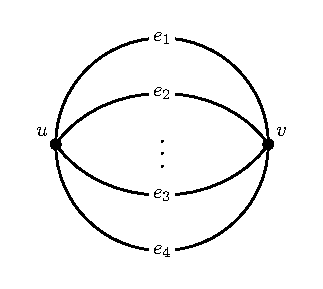
\includegraphics[width=0.32\textwidth]{figures/fig_bundle.pdf}
  \caption{A common-theta bundle of four full lines. The vertices $u$ and $v$ carry no external
  lines, and every line $e_1,\ldots,e_4$ joins this same pair of vertices, hence the same pair of
  current components at every stage of the reduction. All four lines therefore carry the identical
  theta argument $\Delta=\tau_u-\tau_v$ and form one bundle $\cB$ with $|\cB|=4$. The two vertices
  sit at the left and the right end, the outer two lines make up the halves of one circle, and the
  vertical dots between the inner two lines stand for any number of further lines joining the same
  pair, so the bundle is not restricted to the four lines drawn.}
  \label{fig:bundle}
\end{figure}

Write the bundle as, per edge $e$, an ordered pair of endpoint products $\alpha_e$ (coefficient of
$\theta(\Delta)$) and $\beta_e$ (coefficient of $\theta(-\Delta)$).
\begin{enumerate}
  \item \emph{Multiply the thetas out first.} Since inside a bundle all thetas are the same
        function, $\theta(\Delta)^2=\theta(\Delta)$ and $\theta(\Delta)\theta(-\Delta)=0$, the
        product of $|\cB|$ lines collapses to \emph{two} terms rather than $2^{|\cB|}$,
        \begin{equation}
          \prod_{e\in\cB}\Big(\theta(\Delta)\alpha_e+\theta(-\Delta)\beta_e\Big)
          =\theta(\Delta)\prod_{e\in\cB}\alpha_e
          +\theta(-\Delta)\prod_{e\in\cB}\beta_e .
          \label{eq:bundle-two-terms}
        \end{equation}
  \item \emph{One theta, one delta.} Differentiating the shared theta yields a single
        $\delta(\Delta)$ whose coefficient is the antisymmetric difference under
        $\alpha\leftrightarrow\beta$,
        $\partial_\Delta\big[\theta(\Delta)\prod\alpha_e+\theta(-\Delta)\prod\beta_e\big]
        =\delta(\Delta)\big(\prod_e\alpha_e-\prod_e\beta_e\big)$, so all contact information of
        the bundle is concentrated in one distribution and the endpoints are forced to coincide
        only once.
  \item \emph{Split and change basis.} Telescoping the antisymmetric difference and then collecting
        in $\mathsf d_e=\alpha_e-\beta_e$ and $\mathsf m_e=(\alpha_e+\beta_e)/2$ leaves only terms
        with an odd number of $\mathsf d$ factors, each with a numerical coefficient,
        \begin{equation}
          \prod_{e\in\cB}\alpha_e-\prod_{e\in\cB}\beta_e
          =\sum_{\substack{\varnothing\neq S\subseteq\cB\\|S|\ \mathrm{odd}}}
          2^{1-|S|}\prod_{e\in S}\mathsf d_e\prod_{e\notin S}\mathsf m_e .
          \label{eq:bundle-odd-subsets}
        \end{equation}
  \item \emph{Read off the events.} Every non-empty odd subset $S$ is one simultaneous contact
        event: the edges of $S$ are contracted at once, their endpoints merge once, the component
        count drops by one, and the base power of the merged component follows
        \eqref{eq:base-power} with $|C|-1$ merge terms. The injection matrix
        $C^{(v,1)}_{st}$ of \eqref{eq:contact-injection} for such an event is the tensor product of
        the local selectors of the edges in $S$, multiplied by $2^{1-|S|}$ and by the spectator
        factors $\mathsf m_e$.
\end{enumerate}
The collected form \eqref{eq:bundle-odd-subsets} rather than the term-by-term telescoping is what
the program uses, because a term-by-term enumeration would count the same sector transition
several times; the argument, the parity proof and the treatment of unselected edges whose endpoints
become coincident are given in App.~\ref{app:theta}.



\section{Using the package}
\label{sec:usage}

\subsection{Installation and loading}
\label{sec:overview}

Before using package we collect the system requirements and the loading commands.

\paragraph{System requirements.}
\begin{itemize}
  \item A Wolfram Language kernel: Mathematica or the free Wolfram Engine (the package is a
        \texttt{.wl} package; no external Wolfram libraries are needed).
  \item Python 3.10 or newer with \texttt{python-flint>=0.6} and \texttt{sympy>=1.12} installed, for the numerical backend.
        MadStree follows a zero-probe policy: the interpreter is selected only by the explicit
        \texttt{PythonExecutable} option or, when that is \texttt{Automatic} (the default), by the
        \texttt{MADSTREE\_PYTHON} environment variable, falling back to \texttt{"python"}.
\end{itemize}
Install the dependencies in the Python interpreter used for numerical evaluation:
\begin{verbatim}
python -m pip install "python-flint>=0.6" "sympy>=1.12"
\end{verbatim}
Here \texttt{python} should be replaced by the selected interpreter if necessary.
MadStree includes a copy of FlintNDE under \texttt{MadStree/Vendor/FlintNDE},
so a separate installation of the FlintNDE package is not required.

\paragraph{Loading the package.}

Download or clone the official release repository
\url{https://github.com/J7C/dSIBP-Packages}, which contains \texttt{dSIBP}, \texttt{MadStree} and
\texttt{FlintNDE}.
Set \texttt{madStreeDirectory} to the \texttt{MadStree} directory in the local repository,
add it to \texttt{\$Path}, and load with \texttt{Needs}:
\begin{verbatim}
madStreeDirectory = ".../dSIBP-Packages/MadStree";
AppendTo[$Path, madStreeDirectory];
Needs["MadStree`"];
\end{verbatim}
Replace the example path with the absolute path to the local \texttt{MadStree} directory.
This loads \texttt{MadStree.m}, which loads \texttt{Kernel/MadStree.wl} with explicit UTF-8.
Equivalently, load the kernel file directly:
\begin{verbatim}
Get[FileNameJoin[{madStreeDirectory, "Kernel", "MadStree.wl"}],
  CharacterEncoding -> "UTF-8"];
\end{verbatim}
Loading through \texttt{Needs} requires no user encoding option.
MadStree uses its bundled FlintNDE backend without requiring \texttt{Needs["FlintNDE`"]}.
Use a fresh kernel when switching versions, since \texttt{Needs} does not reload
an already loaded package.

After loading, \texttt{MSFlintNDEConfiguration[]} returns
an association. The following expression should return \texttt{"1.0"}:
\begin{verbatim}
MSFlintNDEConfiguration[]["version"]
\end{verbatim}
The following expression should return \texttt{True}:
\begin{verbatim}
MSFlintNDEConfiguration[]["availableQ"]
\end{verbatim}
It confirms that \texttt{flintnde/\_\_init\_\_.py} exists under the configured backend
directory, which is \texttt{Vendor/FlintNDE} relative to \texttt{madStreeDirectory} by default.

\subsection{Input formats and core functions}
\label{sec:inputs}

\paragraph{Tree diagrams: \texttt{MSInitTree}.}

A tree is given by an association of vertices and lines,
\begin{verbatim}
spec = <|
  "name" -> "masslessFullEdge",
  "vertices" -> {
    <|"id" -> v1, "externalLegEnergy" -> k1,
      "timePower" -> a1, "vertexType" -> "+"|>,
    <|"id" -> v2, "externalLegEnergy" -> k2,
      "timePower" -> a2, "vertexType" -> "+"|>
  },
  "lines" -> {
    <|"type" -> "massless", "endpoints" -> {v1, v2},
      "momentum" -> q, "nu" -> 1/2|>
  }
|>;
context = MSInitTree[spec];
\end{verbatim}
Vertex fields:
\begin{center}
\begin{tabular}{@{}lp{5.5cm}p{3.8cm}@{}}
\toprule
field & meaning & note\\
\midrule
\texttt{id} & vertex symbol & required\\
\texttt{externalLegEnergy} & external energy parameter (e.g.\ \texttt{k1}) & optional; default $0$\\
\texttt{timePower} & time-power variable $a_v$ (e.g.\ \texttt{a1}) & required\\
\texttt{vertexType} & contour assignment \texttt{"+"} or \texttt{"-"} & required\\
\bottomrule
\end{tabular}
\end{center}
Line fields:
\begin{center}
\begin{tabular}{@{}p{4.4cm}p{5.3cm}p{3.8cm}@{}}
\toprule
field & meaning & note\\
\midrule
\texttt{type} & \texttt{"massive"} or \texttt{"massless"} & required\\
\texttt{endpoints} & list of one external or two internal vertex endpoints & required\\
\texttt{momentum} & momentum variable $k_i$ (e.g.\ \texttt{q}) & required\\
\texttt{nu} & supplied Bessel/Hankel order $\nu$ & required for massive lines; massless default $1/2$\\
\bottomrule
\end{tabular}
\end{center}
A massless line joining two internal vertices is classified internally as \texttt{masslessFull} and
always uses the shared two-state quotient basis of Sec.~\ref{sec:dlog}; there is no field that
selects another massless representation.
The initialization option \texttt{NuConvention -> "Positive"} (default) or \texttt{"Negative"}
chooses the prefactor sign of $h(\nu,0;z)=z^{\pm\nu}H_\nu(z)$ introduced in
Sec.~\ref{sec:conventions}; it is fixed for the whole context and cannot be changed per call.

Line numbers are assigned from the input order. The Full, Cross or External class and the contour signs are derived from the \texttt{vertexType} of the endpoint vertices; they are not supplied as line types or as separate sign fields. A \texttt{"+"} vertex has phase $e^{-\ii E\tau}$ and a \texttt{"-"} vertex has phase $e^{+\ii E\tau}$, where $E$ is \texttt{externalLegEnergy}. An omitted or zero external energy is represented internally by an auxiliary variable whose target value is zero. Full lines that share the same pair of endpoints are grouped into one common-theta bundle automatically; the optional top-level field \texttt{"thetaBundles"} pins such a group explicitly as a list of line ids, and any group whose members do not share one endpoint pair is rejected.
\paragraph{Loop diagrams without loop integral: \texttt{MSInitTimeGraph}.}

For a pure time-order graph the vertex and line fields are the same, but the graph may contain
cycles. A triangle cycle reads
\begin{verbatim}
cycleContext = MSInitTimeGraph[<|
  "vertices" -> {
    <|"id" -> t1, "externalLegEnergy" -> k1,
      "timePower" -> a1, "vertexType" -> "+"|>,
    <|"id" -> t2, "externalLegEnergy" -> k2,
      "timePower" -> a2, "vertexType" -> "+"|>,
    <|"id" -> t3, "externalLegEnergy" -> k3,
      "timePower" -> a3, "vertexType" -> "+"|>
  },
  "lines" -> {
    <|"type" -> "massless", "endpoints" -> {t1, t2},
      "momentum" -> q12, "nu" -> 1/2|>,
    <|"type" -> "massless", "endpoints" -> {t2, t3},
      "momentum" -> q23, "nu" -> 1/2|>,
    <|"type" -> "massless", "endpoints" -> {t3, t1},
      "momentum" -> q31, "nu" -> 1/2|>
  }
|>];
\end{verbatim}
Here every line joins two internal vertices, so all three are classified internally as
\texttt{masslessFull}. Once one of them is contracted, the remaining two connect the same pair of
components and therefore form the common-theta bundle of Sec.~\ref{sec:common-theta}.

\paragraph{Single-vertex integral families: \texttt{MSInitVertexFamily}.}

No fake topology is needed for a single vertex. The compact input follows the reference
\texttt{ki/nui} convention,
\begin{verbatim}
vertexContext = MSInitVertexFamily[<|
  "ki" -> {k0, k1, k2},
  "nui" -> {a0, nu1, nu2},
  "hankelBranches" -> {1, 2}
|>, NuConvention -> "Positive"];
\end{verbatim}
where \texttt{First[ki]} is the pure vertex phase energy and \texttt{First[nui]} the base power of
$(-\tau)$; the remaining entries give, position by position, the $h$-block momenta and their Hankel
orders $\nu$, which are used verbatim as in Sec.~\ref{sec:conventions}. The explicit alternative
\texttt{externalLegEnergy/timePower/hBlocks/exponentialBlocks} is also accepted, where each
$h$-block is an association with the keys \texttt{momentum}, \texttt{nu} and
\texttt{hankelBranch}. Unlike tree and time-graph input, \texttt{MSInitVertexFamily} rejects any
field outside its own key set.

\paragraph{Package conventions.}
\label{sec:package}

The package implements the $h$-states of \eqref{eq:h-definition} with $z=-k\tau$ and the
single function name $h$, using
\begin{equation}
  h(\nu,0;z)=z^{\pm\nu}H_\nu(z),
  \label{eq:positive-order-h}
\end{equation}
where the plus sign is the default (\texttt{NuConvention->"Positive"}) and the minus sign gives
the convention of \cite{Chen:2023iix}; the two bases are related by $\nu\to-\nu$
(Sec.~\ref{sec:conventions}). The master integrals are the $I_{\tilde{\bm a}}$ of
\eqref{eq:vertex-integral-family}; for multi-vertex correlators they are the products and
sub-sector integrals of Sec.~\ref{sec:dlog}. Each master integral is represented by
\texttt{MSIntegral[sectorKey, timeShifts, stateBits]}: \texttt{sectorKey} is a binary string over
the root lines in the input order, with \texttt{1} for a line that is still active and
\texttt{0} for a line contracted by a contact; \texttt{timeShifts} assigns one integer shift of
the base time power to every vertex component, where a component is a maximal set of vertices
merged by the contractions; \texttt{stateBits} gives the state of every two-state slot of the
sector in the slot order. {\color{red}The master integrals are the entries with vanishing shifts}, and their
connection is the d log-form \eqref{eq:ndlogDE} of Sec.~\ref{sec:dlog}.

Let us see some examples for $\texttt{MSIntegral[sectorKey, timeShifts, stateBits]}$. For the three-vertex chain $v_1$--$v_2$--$v_3$ with internal lines $l_{12}$, $l_{23}$, vertex
energies $k_1,k_2,k_3$ and time powers $a_1,a_2,a_3$, the contact-reachable sectors are the four
strings \texttt{"11"}, \texttt{"01"}, \texttt{"10"}, \texttt{"00"},
\begin{center}
\emph{(i) both lines massive: $l_{12}$ with $\nu_{12}$, $l_{23}$ with $\nu_{23}$.}\\[2pt]
\footnotesize\begin{tabular}{@{}lllp{5.8cm}@{}}
\toprule
\texttt{sectorKey} & contracted & components & master integrals\\
\midrule
\texttt{"11"} & --- & $\{v_1\},\{v_2\},\{v_3\}$
  & \texttt{MSIntegral["11",\{0,0,0\},\{a,b,c,d\}]} (16)\\
\texttt{"01"} & $l_{12}$ & $\{v_1,v_2\},\{v_3\}$
  & \texttt{MSIntegral["01",\{0,0\},\{c,d\}]} (4)\\
\texttt{"10"} & $l_{23}$ & $\{v_1\},\{v_2,v_3\}$
  & \texttt{MSIntegral["10",\{0,0\},\{a,b\}]} (4)\\
\texttt{"00"} & $l_{12},l_{23}$ & $\{v_1,v_2,v_3\}$
  & \texttt{MSIntegral["00",\{0\},\{\}]} (1)\\
\bottomrule
\end{tabular}
\end{center}
\begin{center}
\emph{(ii) $l_{12}$ massive with $\nu_{12}$, $l_{23}$ massless.}\\[2pt]
\footnotesize\begin{tabular}{@{}lllp{5.8cm}@{}}
\toprule
\texttt{sectorKey} & contracted & components & master integrals\\
\midrule
\texttt{"11"} & --- & $\{v_1\},\{v_2\},\{v_3\}$
  & \texttt{MSIntegral["11",\{0,0,0\},\{a,b,r\}]} (8)\\
\texttt{"01"} & $l_{12}$ & $\{v_1,v_2\},\{v_3\}$
  & \texttt{MSIntegral["01",\{0,0\},\{r\}]} (2)\\
\texttt{"10"} & $l_{23}$ & $\{v_1\},\{v_2,v_3\}$
  & \texttt{MSIntegral["10",\{0,0\},\{a,b\}]} (4)\\
\texttt{"00"} & $l_{12},l_{23}$ & $\{v_1,v_2,v_3\}$
  & \texttt{MSIntegral["00",\{0\},\{\}]} (1)\\
\bottomrule
\end{tabular}
\end{center}
\begin{center}
\emph{(iii) both lines massless.}\\[2pt]
\footnotesize\begin{tabular}{@{}lllp{5.8cm}@{}}
\toprule
\texttt{sectorKey} & contracted & components & master integrals\\
\midrule
\texttt{"11"} & --- & $\{v_1\},\{v_2\},\{v_3\}$
  & \texttt{MSIntegral["11",\{0,0,0\},\{r,s\}]} (4)\\
\texttt{"01"} & $l_{12}$ & $\{v_1,v_2\},\{v_3\}$
  & \texttt{MSIntegral["01",\{0,0\},\{r\}]} (2)\\
\texttt{"10"} & $l_{23}$ & $\{v_1\},\{v_2,v_3\}$
  & \texttt{MSIntegral["10",\{0,0\},\{r\}]} (2)\\
\texttt{"00"} & $l_{12},l_{23}$ & $\{v_1,v_2,v_3\}$
  & \texttt{MSIntegral["00",\{0\},\{\}]} (1)\\
\bottomrule
\end{tabular}
\end{center}


The vertex \texttt{vertexType} field (\texttt{"+"} or \texttt{"-"}) determines the sign of the pure
vertex exponential $e^{\ii k_0\tau}$ of \eqref{eq:vertex-integral-family}, and the pair of endpoint
types determines the SK class of each line, from which the default Hankel branches of
\eqref{eq:h-definition} follow; a line may override them with its own \texttt{hankelBranches}
field. The
package $h$-states are those of \eqref{eq:h-definition}, i.e.\
$h(\nu,1;z)=\partial_zh(\nu,0;z)$, with the alternative prefactor $z^{+\nu}$ obtained by
$\nu\to-\nu$; \texttt{MSHTohMatrix}, \texttt{MShToHMatrix} and \texttt{MSConvertBasis}
implement the corresponding basis change and its Kronecker products, with the massless shared
two-state of Sec.~\ref{sec:massless} acting trivially on the reduced states.



Once the context is initialized, the following functions expose the formula products of Sec.~\ref{sec:method}.

\paragraph{Core functions.}
\label{sec:core}

Most functions take the initialized \texttt{context};
\texttt{MSExportEvaluationData} takes a completed evaluation result instead.

\begin{center}
\begin{tabular}{@{}p{7.1cm}p{7.3cm}@{}}
\toprule
function & purpose\\
\midrule
\texttt{MSSectors[context]} & contact-reachable sectors in deterministic order (keys, pinched
lines, master counts)\\
\texttt{MSMasterIntegrals[context]} & ordered master records; each \texttt{"integral"} field is an
\texttt{MSIntegral[sectorKey, timeShifts, stateBits]}\\
\texttt{MSFormulaMatrices[context, key]} & per-component $\text{M}_1$, $\text{M}_0$ and energy letters $\kappa_{\bm a}$;
sector diagonalizer \texttt{U} and \texttt{UInverse}\\
\texttt{MSDLogDE[context]} & block-triangular d log-form potential $\Omega$, letters, certification
status\\
\texttt{MSReduce[expr, context]} & iterative IBP reduction to the master basis; scalar, list or nested table input\\
\texttt{MSContactMaps[context, key]} & parent-to-sub-sector contact maps\\
\texttt{MSWriteFormulaArtifacts[context]} & write formula products beside the caller\\
\texttt{MSFormulaData[context]} & aggregate all-sector masters, recurrence metadata and the d log-form DE\\
\texttt{MSEvaluatePath[context, pointSequence, opts]} & single-stage evaluation: boundary initialization and segment transport in one backend process; optional FlintNDE path planning\\
\texttt{MSReconstructEpSeries[context, ep, pointSequence, opts]} & Laurent series in the common analytic regulator: certified lowest power, automatic sample points, incremental fitting\\
\texttt{MSExportEvaluationData[evaluation, opts]} & export the saved ordinary-point records of an evaluation to CSV/JSON\\
\bottomrule
\end{tabular}
\end{center}

\begin{description}
  \item[\texttt{MSSectors[context]}] returns the sector list. Each sector key is the fixed-length
        bit string over the root lines in input order (\texttt{"0"} pinched, \texttt{"1"} unpinched); the
        sub-sector structure is discussed in Sec.~\ref{sec:dlog}. Keys are
        strings, not integers; leading zeros are part of the identity.
  \item[\texttt{MSMasterIntegrals[context]}] returns the ordered master records.
        Their \texttt{"integral"} fields contain the
        \texttt{MSIntegral[sectorKey, timeShifts, stateBits]} objects of Sec.~\ref{sec:package}, i.e.\
        the master integrals $I_{\tilde{\bm a}}$ of \eqref{eq:vertex-integral-family}.
        Use \texttt{Lookup[MSMasterIntegrals[context], "integral"]} to obtain this ordered basis.
        Each record also contains \texttt{"bareIntegral"}, \texttt{"normalization"} and
        \texttt{"definition"}. Their order is the unique authority for all matrices, boundary
        vectors and numerical results.
  \item[\texttt{MSFormulaMatrices[context, key]}] returns the component records under
        \texttt{"components"}, with fields \texttt{"M1"}, \texttt{"M0"} and
        \texttt{"energyLetters"} for the matrices and letters of Sec.~\ref{sec:global}.
        The sector diagonalizer of $\text{M}_0$ and its inverse are returned as
        \texttt{"U"} and \texttt{"UInverse"}; $\text{M}_1$ is already diagonal in the state basis.
        Here \texttt{key} is a sector-key string; omitting it, or passing \texttt{All},
        returns an association for all sectors. \texttt{MSContactMaps} accepts the same
        sector selection.
  \item[\texttt{MSDLogDE[context]}] returns \texttt{omegaPotential}, the matrix $\Omega$ of
        Sec.~\ref{sec:dlog} whose derivative along a path is the DE matrix, together with the
        letters (the arguments of the logarithms of \eqref{eq:omega-form}),
        \texttt{letterMatrices}, \texttt{dlogResidual}, \texttt{constantResidueQ} and the
        certification \texttt{dlogStatus}. Only \texttt{"certifiedByFormulaChecks"} is a closed
        d log-form and may be consumed numerically.
  \item[\texttt{MSReduce[expr, context, MasterBasis -> Automatic]}] reduces finite linear
        combinations of legal \texttt{MSIntegral}s, or lists and nested tables of such
        expressions, by
        the lowering/raising recurrences $A_\pm$ of Sec.~\ref{sec:global} along the
        sub-sector structure of Sec.~\ref{sec:dlog}. Results include
        \texttt{result}, \texttt{masterBasis}, \texttt{coefficientVector}, \texttt{masterRules},
        \texttt{nonMasterResidual}, \texttt{remainingShiftedIntegrals} and
        \texttt{singularLayers}; a full reduction requires a zero residual and an empty shifted
        list for every scalar expression. For list input, these fields preserve the input
        shape; \texttt{elementResults}, \texttt{failurePositions} and
        \texttt{incompletePositions} provide the element-level reports.
  \item[\texttt{MSFormulaData[context]}] returns all-sector masters, the per-sector
        $\text{M}_1/\text{M}_0/\text{T}_n$ recurrence metadata of Sec.~\ref{sec:global} and the complete
        block-triangular d log-form DE in the master order of \texttt{MSDLogDE};
        \texttt{TimePowerRules} may substitute the vertex time powers $a_i$ in the recurrence
        metadata, but the returned \texttt{"dlogDE"} remains analytic and unsubstituted.
  \item[\texttt{MSEvaluatePath[context, pointSequence, opts]}] is the single-stage numerical
        entry for evaluating the master integrals at the user points.
        \texttt{pointSequence} is a coordinate table: its first row gives the ordered
        coordinate symbols and subsequent rows give equal-width coordinate values.
        Fixed parameters are supplied once through \texttt{ParameterRules}. Boundary generation,
        transport and result records are described in Sec.~\ref{sec:numerics}; the principal
        options and point tags are summarized in Sec.~\ref{sec:options}.
  \item[\texttt{MSReconstructEpSeries[context, ep, pointSequence, opts]}] reconstructs the Laurent
        series of the master integrals in a common analytic regulator \texttt{ep}, with
        \texttt{MaximumEpPower} the highest returned power (default $0$, i.e.\ the pole terms and
        the finite part). It uses the same \texttt{pointSequence} and \texttt{ParameterRules}
        format as \texttt{MSEvaluatePath}. Only \texttt{ParameterRules}, not the coordinates,
        may depend on \texttt{ep}. By default, no \texttt{ep} values need to be supplied;
        \texttt{EpSamplePoints} and \texttt{EpValidationPoints} may instead specify production
        candidates and disjoint validation points. The certificate conditions,
        sampling and fitting procedure are described in Sec.~\ref{sec:regulator}; the corresponding
        options are summarized in Sec.~\ref{sec:options}.
  \item[\texttt{MSExportEvaluationData[evaluation, opts]}] exports the saved ordinary-point
        records of one \texttt{MSEvaluatePath} result, including the coordinates, the
        real/imaginary parts of every master, \texttt{status}, \texttt{relativeDifferenceInf} and
        \texttt{targetRelativeErrorMet}, to CSV and JSON for downstream plotting tools; transient
        records are excluded. The two precision fields are the corresponding segment reports,
        not separate error estimates computed at every point. \texttt{ExportFormats} selects
        CSV, JSON or both, and \texttt{SignificantDigits} defaults to $16$;
        see Sec.~\ref{sec:outputs}.
\end{description}

\paragraph{Output organization.}
\label{sec:outputs}

\begin{itemize}
  \item Transient request JSON and backend logs:
        \texttt{results\_temp/\allowbreak nde/} beside the caller by default.
        Request and log files are deleted after a successful run and retained for backend
        failures; structured singular-path or leading-order refusals also remove these files.
        Successful JSON results remain in \texttt{results\_temp/\allowbreak cache/} for reuse.
        \texttt{MSRuntimeDirectory} may specify a different runtime directory.
  \item Saved point records: \texttt{MSEvaluatePath} returns the records under
        \texttt{"pointResults"}. An ordinary untagged coordinate row has
        \texttt{"status" -> "saved"}; \texttt{"saved"} is a status value, not a top-level key.
        A row \texttt{\{\{values...\}, "tmp"\}} gives a transient waypoint, represented by
        \texttt{"status" -> "transient"} and excluded from export.
        Singular-point classifications are returned under \texttt{"singularityClassifications"}
        by the same backend evaluation run.
  \item Formula artifacts: \texttt{MSWriteFormulaArtifacts[context]} writes \texttt{masters.wl},
        \texttt{recurrence\_metadata.wl}, \texttt{dlog\_de.wl} and \texttt{manifest.wl} to
        \texttt{results/\allowbreak madstree\_formula/\allowbreak run-UUID/} by default.
        \texttt{MSEvaluatePath} and \texttt{MSReconstructEpSeries} automatically write or reuse
        these analytic files before numerical transport and return their paths under
        \texttt{"formulaArtifacts"}.
  \item Evaluation export: \texttt{MSExportEvaluationData[result, MSOutputDirectory -> ...]} writes
        \texttt{evaluation\_data.csv} and \texttt{evaluation\_data.json} under
        the caller-chosen output directory (default
        \texttt{results/\allowbreak madstree\_evaluation/\allowbreak run-UUID/}), for downstream
        plotting tools.
  \item Cache identity: a successful-result cache key includes the request and the SHA-256
        identities of the backend adapter, the configured backend's \texttt{pyproject.toml}
        and sorted \texttt{flintnde/*.py}, so
        in-place source fixes invalidate stale cache entries automatically.
\end{itemize}
The package source directory never receives run artifacts.


\subsection{Numerical evaluation}
\label{sec:numerics}

With an initialized context, numerical evaluation proceeds in two steps: boundary generation and
transport. The workflow is single-stage: \texttt{MSEvaluatePath} partitions the user point
sequence into maximal consecutive complex-affine one-variable segments, pulls the d log-form
connection back once per segment, and sends all segments, the exact boundary conditions and the
user options to FlintNDE in one UTF-8 JSON request. With the default
\texttt{FlintNDEPathPlanning -> True}, FlintNDE plans the transport nodes inside each segment and
evaluates user points by fast multipoint evaluation; with \texttt{False} it uses every supplied
point as a node in input order, without inserting, removing, or replanning points. The backend
inside the version directory is a synchronized copy of the standalone \texttt{FlintNDE} package
released in the same repository, whose mechanisms
are described below. \texttt{MSBoundaryData} and \texttt{MSEvaluatePath}
default to 200 decimal working digits; an explicit \texttt{WorkingPrecision} overrides the
default.

\paragraph{Boundary generation.}

\begin{verbatim}
targetRules = {k1 -> 9 I, k2 -> 3 I, q -> 1, a1 -> 1, a2 -> 1};

certificate = MSBoundaryChartCertificate[context, targetRules,
  RankOrder -> All];

boundary = MSBoundaryData[context, targetRules,
  BoundaryScale -> 4, WorkingPrecision -> 200];
\end{verbatim}
\texttt{MSBoundaryChartCertificate} verifies the nested blow-up chart of Sec.~\ref{sec:boundary}
(normal crossing, theta fixing, quotient checks) for the chosen strict energy rank;
\texttt{RankOrder -> All} checks every strict chart. \texttt{MSBoundaryData} consumes the
certificate and returns the leading Frobenius data at the $K_v\to\infty$ boundary: for every master
whose leading weight does not vanish, one branch record carrying the Frobenius exponent, the overall
coefficient and the normalized leading vector, together with the anchor rules, the rank order and
the certificate itself.
If the chart is not certified, it returns \texttt{BoundaryChartNotCertified} and does not proceed
to numerics. The energies in the example are positive imaginary so that the vertex factors
$e^{-\ii E\tau}$ damp at $\tau\to-\infty$; the rank order of the boundary is derived from the
supplied target point, largest damping energy first, unless \texttt{RankOrder} fixes it. The
example passes \texttt{WorkingPrecision -> 200} explicitly; 200 is also the
default, and any explicit positive value overrides it.

\paragraph{Transport.}

\begin{verbatim}
pointSequence = {{k1, k2}, {9 I, 3 I}};
parameterRules = {q -> 1, a1 -> 1, a2 -> 1};

result = MSEvaluatePath[context, pointSequence,
  ParameterRules -> parameterRules,
  BoundaryScale -> 4, RankOrder -> {v1, v2},
  WorkingPrecision -> 200, TransportOrder -> 80,
  ReferenceTransportOrder -> 104,
  TargetRelativeError -> "1e-20",
  MessageLanguage -> "EN"];

result["pointResults"]
\end{verbatim}
The second argument is the \emph{point sequence}: its first row lists the movable coordinate
symbols, and every further row supplies one numerical value for each of them, in the same order.
The remaining symbols of the target point, here \texttt{q}, \texttt{a1} and \texttt{a2}, are fixed
once for the whole run through \texttt{ParameterRules}. For several targets, append one row per
point,
\begin{verbatim}
pointSequence = {{k1, k2}, {8 I, 2 I}, {7 I, 4 I}, {6 I, 5 I}};
\end{verbatim}
and MadStree groups the
points into maximal consecutive complex-affine lines and pulls each group back once, while FlintNDE
evaluates every point in one process, including dense points inside a node's convergence disk,
without changing the path. For a single-vertex integral family, run the same single-stage entry on
the vertex context. The principal transport options and the point tags are summarized in
Sec.~\ref{sec:options}. If every d log-form letter is constant on a segment, every
pulled-back derivative vanishes; the segment is then a zero connection with no finite poles and
is transported normally.

\paragraph{Reading the result.}

\texttt{result} is an association whose \texttt{"pointResults"} entry is the list of point records.
Every saved ordinary point carries
\texttt{coordinate}, \texttt{value} (the master vector in master order), \texttt{status} (equal to
\texttt{"saved"} for ordinary points) and \texttt{userIndex}; transient \texttt{"tmp"} points
participate only in the path. The current version does not provide leading-order point labels:
every tag other than \texttt{"tmp"} is rejected. With the default
\texttt{SingularityMode -> "Automatic"} a segment that meets a supported singularity is crossed by
an explicit jump; \texttt{"Avoid"} refuses such a segment instead, and with
\texttt{FlintNDEPathPlanning -> False} the backend is forced into avoid mode, so a user chain that
crosses a pole or leaves a local convergence disk fails explicitly. The exported per-point
\texttt{relativeDifferenceInf} and \texttt{targetRelativeErrorMet} are obtained from the embedded
truncation certification of Sec.~\ref{sec:backend}, not from a second independent transport chain.
A route-robust access to a saved value is
\begin{verbatim}
savedPoints = Select[result["pointResults"], #["status"] === "saved" &];
firstPoint = First[savedPoints];
firstPoint["value"]
\end{verbatim}

\paragraph{The numerical backend.}
\label{sec:backend}

FlintNDE is a general solver for first-order matrix differential equations with exact
$Q(\ii)(s)$-coefficient systems; MadStree embeds a synchronized copy and only
ever feeds it single-variable pullbacks of the d log-form connection. Three mechanisms are responsible
for the current performance:
\begin{itemize}
  \item \emph{Pole--residue transport.} An ordinary segment is serialized as its pole--residue
        representation $A(x)=P(x)+\sum_jR_j/(x-p_j)$, with $P$ of arbitrary degree and the residues
        $R_j$ of coincident letters merged. The backend generates the solution Taylor coefficients
        by a pole-state recurrence, avoiding the Cauchy sampling and discrete-Fourier coefficient
        reconstruction of a generic analytic-matrix backend.
  \item \emph{Embedded truncation certification.} Only one transport chain is run
        (\texttt{certificationMode -> "embedded"}); the primary result is re-evaluated from the
        coefficient prefix by Horner, and the per-segment truncation difference is returned as a
        local error estimate, so the reference-chain overhead is removed while the
        \texttt{relativeDifferenceInf} and \texttt{targetRelativeErrorMet} fields remain available
        for the user.
  \item \emph{Fast multipoint evaluation.} With \texttt{FlintNDEPathPlanning -> True}, FlintNDE
        plans nodes inside each segment; user points covered by one expansion node form an
        evaluation bucket and are evaluated from the cached vector series. Buckets with at least
        eight points use the subproduct/remainder tree of fast multipoint evaluation, and small
        buckets use the iterative algorithm to avoid tree overhead. User points in the same
        complex-affine group $x(s)=x_0+s\,v$ share node coefficients whenever they lie in the same
        convergence disk; different segments never share local coefficients.
\end{itemize}
Singularity handling is explicit: the default \texttt{SingularityMode -> "Automatic"} maps to the
backend jump mode, so a segment that meets a supported singularity is crossed by an explicit
local-basis jump instead of being refused or detoured; \texttt{"Avoid"} refuses such a segment, and
\texttt{"SingularityJump"} requests a jump unconditionally. Both jump modes are available only when
\texttt{FlintNDEPathPlanning -> True}; with planning disabled the backend is forced into avoid mode
and the user must supply a valid ordinary-point node chain. The branch reached by a jump is fixed
by the local basis and by the winding of the path, and the user must check that it is the intended
one. Exact Lee--Moser balances,
strictly decoupled exponential times, and power-log recurrences are handled, while resonances
whose local bases cannot be constructed, and any ramification or general Stokes requirement, fail
closed. The internal working bits are $\lceil\mathrm{WP}\log_2 10\rceil+32$ for
\texttt{WorkingPrecision} = WP digits (the default WP is 200), and all path geometry (segment
projections, match ratios, rotation factors, winding/monodromy) is kept in Arb/Acb precision.
If the backend realification writes $k=-\ii\kappa$, then $-k^2=+\kappa^2$; a program token
named \texttt{ik} then denotes the real variable $\kappa$, and \texttt{ik\^{}2} is its square,
not the imaginary unit times $k^2$.

\subsection{Laurent-series reconstruction}
\label{sec:regulator}

When all vertex time powers share a common analytic regulator $\varepsilon$, e.g.\
$a_v=1+\varepsilon$, the master integrals develop a Laurent series
\begin{equation}
  I(\varepsilon)=\sum_{p=n_{\min}}^{m}c_p\,\varepsilon^p
  +O(\varepsilon^{m+1}),
  \label{eq:regulator-laurent}
\end{equation}
and \texttt{MSReconstructEpSeries[context, ep, pointTemplate, MaximumEpPower -> m]}
reconstructs the coefficients $c_{n_{\min}},\ldots,c_m$. The user supplies no
$\varepsilon$ values; the lowest power is not a numerical fit parameter.

\paragraph{Certification of the lowest power.}
Before any numerical solve at nonzero $\varepsilon$, MadStree constructs a support
certificate from the symbolic boundary conditions and the d log-form DE of the production
context. It requires:
\begin{enumerate}
  \item regulator-independent path coordinates and no negative Laurent power at
        $\varepsilon=0$ in any d log-form matrix, pulled-back connection, or residue;
  \item finite-Laurent boundary branches, where branches with the same limiting Frobenius
        exponent and log degree are first combined with their physical weights and leading
        vectors, and only then are component valuations extracted;
  \item at least one provably nonzero coefficient at the lowest power of the combined
        boundary; a noninteger power, non-Laurent structure, undecidable coefficient, or
        support entirely above the requested user range fails closed.
\end{enumerate}
For $n_{\min}<0$ the certificate describes a finite meromorphic Laurent boundary, not an
analytic boundary at $\varepsilon=0$; analyticity is recorded only when $n_{\min}\geq0$.
Along the current finite path an $\varepsilon$-analytic invertible fundamental matrix
preserves the valuation of nonzero formal boundary conditions, so the certified $n_{\min}$ is
passed directly to the sampling plan. A rank drop of an individual Frobenius recurrence
operator at $\varepsilon=0$ is retained as a resonance diagnostic only; it is not by itself
interpreted as a $1/\varepsilon$ pole of the already combined physical boundary.

\paragraph{Sampling, fitting and validation.}
Given the highest requested power $m$ and the certified lowest power $n_{\min}$, the plan sets
\begin{equation}
  P=\max(0,-n_{\min}),\qquad
  \Delta=m-n_{\min},\qquad
  N_{\rm fit}=\max\!\left(\left\lceil\tfrac52\Delta+P\right\rceil,\Delta+1\right),
  \label{eq:regulator-fit-count}
\end{equation}
and chooses the $\varepsilon$ scale and precisions
\begin{equation}
  \alpha_\varepsilon=\frac{P}{4}+\frac{g}{\Delta+1},\qquad
  \varepsilon_0=10^{-\alpha_\varepsilon},\qquad
  p_0=\max\!\left(\left\lceil(N_{\rm fit}+P)\alpha_\varepsilon\right\rceil,30\right),
  \label{eq:regulator-scale-precision}
\end{equation}
where $g=\texttt{EpGoalDigits}$ is the requested decimal accuracy. The working precision is
$\max(200,\lceil2(1+e)p_0\rceil)$ with $e$ the extra-precision fraction; the primary
transport order is $4p_0$ and the reference chain adds
$\lceil\max(50,p_0/5)\rceil$ orders. All $N_{\rm fit}$ production points enter one square
Acb Vandermonde system interpolating through $\varepsilon^{n_{\min}+N_{\rm fit}-1}$; only
$c_{n_{\min}},\ldots,c_m$ are returned, and no least squares or pseudoinverse is used.
Independent validation points are placed at a fixed fraction of the production scale, never
enter the fit, and the truncated series must pass the relative tolerance $10^{-g}$; otherwise
the run fails closed.

\paragraph{Incremental expansion and parallelism.}
The initial fit includes at least two powers above the user maximum
(\texttt{EpFitExtraOrder -> 2}). If validation fails, each subsequent round adds
\texttt{EpFitOrderIncrement -> 2} powers, solves only the new production points, and reuses
every previous production and validation value, for at most \texttt{EpFitMaximumRounds -> 3}
rounds; the tolerance is not relaxed and the caches are not discarded. Independent
$\varepsilon$ tasks run in an outer process pool bounded by \texttt{ParallelTaskCount -> 12},
whose effective concurrency is the smaller of the limit and the number of tasks; this is
separate from the in-process \texttt{ctx.threads} of python-flint.

\subsection{Options, validation and common pitfalls}
\label{sec:options}

The principal options of the numerical workflow are summarized below.
\begin{center}
\begin{tabular}{@{}p{5.0cm}p{9.3cm}@{}}
\toprule
option & meaning\\
\midrule
\texttt{FlintNDEPathPlanning} & \texttt{True} (default): FlintNDE plans nodes and uses fast
multipoint evaluation; \texttt{False}: user points as nodes in input order\\
\texttt{SingularityMode} & \texttt{"Automatic"} (default), \texttt{"Avoid"} or \texttt{"SingularityJump"}\\
\texttt{MessageLanguage} & \texttt{"EN"} (default) or \texttt{"CN"}, case-sensitive\\
\texttt{BoundaryScale} & scale setting the damping energies at the finite boundary anchor ($>1$; default 8)\\
\texttt{BoundarySeriesOrder} & boundary-order metadata and regulator recurrence diagnostics; not the numerical Frobenius start order in the current generic route\\
\texttt{RankOrder} & vertex order by damping energy $K_v$ (default \texttt{Automatic}: from the first target point)\\
\texttt{WorkingPrecision} & integer working precision in decimal digits, at least 20; default 200\\
\texttt{TransportOrder} / \texttt{ReferenceTransportOrder} & primary and reference local-series orders, including the numerical Frobenius start; defaults 48 and 64, with the reference order strictly larger\\
\texttt{TargetRelativeError} & target relative error of the primary/reference check; default \texttt{"1e-25"}\\
\texttt{MaximumEpPower} & highest returned regulator power of \texttt{MSReconstructEpSeries}
(default 0)\\
\texttt{EpGoalDigits} & requested decimal accuracy of the reconstructed regulator coefficients
(default 20)\\
\texttt{EpFitExtraOrder} / \texttt{EpFitOrderIncrement} / \texttt{EpFitMaximumRounds} & internal
buffer powers, per-round increment and maximum refit rounds of the regulator fit (defaults 2, 2, 3)\\
\texttt{ParallelTaskCount} & maximum concurrent \texttt{ep} backend processes in \texttt{MSReconstructEpSeries} (default 12)\\
\texttt{PythonExecutable} & Python command for the FlintNDE adapter (default \texttt{Automatic})\\
\texttt{MSRuntimeDirectory} & temporary-file root (default: \texttt{results\_temp} in the calling script or notebook directory)\\
\bottomrule
\end{tabular}
\end{center}

The transport orders and \texttt{TargetRelativeError} above apply to
\texttt{MSEvaluatePath}. For \texttt{MSReconstructEpSeries}, these three options
are not accepted; the numerical settings are planned from \texttt{EpGoalDigits}.
Its \texttt{BoundarySeriesOrder} defaults to \texttt{Automatic}, whereas
\texttt{MSEvaluatePath} uses 24.

Saved and transient points are not a transport option: they are tags attached to coordinate
rows below the symbol header (bare value lists and \texttt{\{\{values...\},"tmp"\}}).
With \texttt{SingularityMode -> "Avoid"}, interior singularity crossings are refused
and reported with the offending path pairs. The default \texttt{"Automatic"} mode
allows supported singularity jumps when \texttt{FlintNDEPathPlanning -> True};
an explicit \texttt{"SingularityJump"} also requires this setting.
When planning is disabled, \texttt{"Automatic"} uses \texttt{"Avoid"}.
The user must check the selected multivalued branch. An explicitly requested
terminal singular point is handled by local classification and evaluation,
rather than by ordinary Taylor transport through the singularity.


Limitations and fail-closed guarantees:
\begin{itemize}
  \item No loop-momentum integration, no sampled IBP, no Kira or external reduction.
  \item \texttt{dlogStatus} must be \texttt{"certifiedByFormulaChecks"}; otherwise the DE is not
        consumed.
  \item Uncertified boundary charts and singular points beyond the
        backend's certified capabilities all fail closed; resonances whose local bases cannot be
        constructed return structured refusals, and ordinary Taylor transport is never used across
        singular points.
  \item An incomplete \texttt{MSReduce} call may return an association with
        \texttt{"status" -> "partiallyReduced"} or \texttt{"status" -> "failed"},
        rather than a top-level \texttt{Failure}. Inspect
        \texttt{"remainingShiftedIntegrals"} and \texttt{"nonMasterResidual"}.
  \item For \texttt{MSEvaluatePath}, check
        \texttt{result["flintNDE"]["targetRelativeErrorMet"]}, not only
        \texttt{result["status"]}. For \texttt{MSReconstructEpSeries}, check
        \texttt{"precisionTargetMet"}; coefficients may be returned with
        \texttt{"status" -> "computed\_with\_warning"} if the target is not met.
  \item The production boundary never uses defining integrals; finite-point defining integrals
        exist only inside independent validation programs.
\end{itemize}

Finally, we collect the most common mistakes.

\paragraph{Common pitfalls.}
\label{sec:pitfalls}

\begin{enumerate}
  \item \textbf{Convention}: \texttt{NuConvention} is chosen at initialization only
        (\texttt{"Positive"} by default). To compare with the formulas of
        \cite{Chen:2024glu}, initialize with \texttt{NuConvention -> "Negative"}, which selects
        the minus sign in \eqref{eq:positive-order-h}.
  \item \textbf{Sector keys}: fixed-length strings; leading zeros and the string type are part of
        the identity (Sec.~\ref{sec:dlog}).
  \item \textbf{Single-stage workflow}: call \texttt{MSEvaluatePath} directly. \texttt{MadStree} in this version does not
        provide \texttt{MSGeneratePath}, \texttt{MSEvaluatePlannedPath}, public plan objects, old JSON
        schemas or any migration wrapper; the default \texttt{WorkingPrecision} is 200 and an
        explicit value overrides it.
  \item \textbf{Singularity handling}: the default is \texttt{SingularityMode -> "Automatic"},
        where \texttt{"Automatic"} is a string, not the symbol \texttt{Automatic}.
        Use \texttt{"Avoid"} to refuse interior crossings. Supported jumps require
        \texttt{FlintNDEPathPlanning -> True}, and the user must check the multivalued branch.
  \item \textbf{Point tags}: after the coordinate-symbol header, only bare value lists and
        \texttt{\{\{values...\},"tmp"\}} are accepted; every other tag, including
        \texttt{"lo"}, is rejected.
  \item \textbf{Backend environment}: MadStree uses zero probing; the interpreter is given by the
        \texttt{PythonExecutable} option or, when \texttt{Automatic}, by the
        \texttt{MADSTREE\_PYTHON} environment variable (falling back to \texttt{"python"}), and it
        requires Python 3.10 or later with \texttt{python-flint>=0.6} and
        \texttt{sympy>=1.12}, and must be able to import the embedded
        \texttt{flintnde}. Backend failures report captured output through messages such as
        \texttt{backendLaunchFailed} and \texttt{backendRunFailed}; retained runtime logs
        contain the details. Successful calls and handled singular-path refusals remove
        their temporary input and log files.
  \item \textbf{Message language}: \texttt{MessageLanguage} accepts only \texttt{"EN"} and
        \texttt{"CN"} (case-sensitive), with \texttt{"EN"} the default.
  \item \textbf{Encoding}: loading through \texttt{Needs} uses explicit UTF-8 internally and needs
        no user encoding option; if loading the kernel file directly fails with syntax errors, set
        \texttt{\$CharacterEncoding = "UTF-8"} before loading.
\end{enumerate}

\section{Examples}
\label{sec:examples-section}

We reproduce the results for the tree with two vertices and one
massive exchange~\cite{Chen:2024glu} and the tree with three vertices
and two massive exchanges~\cite{Xianyu:2023ytd}.
Further checks cover recurrence reduction, zero external energy,
single vertex families, time graphs, transport accuracy and stability,
and Laurent series reconstruction in the numerical backend.
We also cross check the master definitions and normalizations
with the dSIBP package~\cite{dSIBP:inPreparation}.

We first list the examples shipped with the package and then present two numerical applications.

\subsection{Package examples}
\label{sec:examples}
The distribution ships seven examples that exercise the complete workflow:
\begin{itemize}
  \item \texttt{01\_massless\_full\_edge.wl}: the massless shared two-state simplification of
        Sec.~\ref{sec:massless}, masters, recurrence, d log-form DE and the automatic
        boundary/numerical entry; it also demonstrates the
        single-stage multipoint workflow, with CSV/JSON export;
  \item \texttt{02\_single\_vertex\_family.wl}: single-vertex integral family input, local tensor
        inverses (Sec.~\ref{sec:global}), and finite-combination reduction;
  \item \texttt{03\_time\_only\_cycle\_chart.wl}: time-order cycle input, common-theta contacts
        (Sec.~\ref{sec:common-theta} and App.~\ref{app:theta}), and
        all strict-rank chart certificates; contacts are discussed in Sec.~\ref{sec:dlog};
  \item \texttt{04\_three\_vertex\_tree.wl}: a three-vertex, two-propagator massless tree
        ($+++$ vertex structure), following the same flow as example 01, with a single-stage
        multipoint evaluation and CSV/JSON export;
  \item \texttt{05\_massive\_three\_vertex\_tree.wl}: a three-vertex, two-propagator massive tree
        ($+++$ vertex structure) with non-half-integer \texttt{nu12=3/4}, \texttt{nu23=1/3},
        followed by a single-stage multipoint evaluation and CSV/JSON export;
  \item \texttt{06\_massless\_three\_vertex\_ep\_regularization.wl}: a three-vertex massless tree
        with the common analytic regulator $a_1=a_2=a_3=1+\varepsilon$; the user requests
        only the highest regulator power (\texttt{MaximumEpPower -> 0}), and the program certifies
        the lowest power from the symbolic boundary and DE before choosing production/validation
        points and extracting the pole and finite part;
  \item \texttt{07\_zero\_external\_leg\_energy.wl}: zero external-leg energy, represented through an auxiliary energy with zero target value.
\end{itemize}

In the massless three-vertex example (Example~06) with $a_1=a_2=a_3=1+\varepsilon$, the
physical boundary weights contain $\Gamma(2+\varepsilon)^3$,
$\Gamma(2+\varepsilon)\Gamma(4+2\varepsilon)$ and $\Gamma(6+3\varepsilon)$, all regular at
$\varepsilon=0$, and the nine-dimensional DE has no negative $\varepsilon$ power; the
certificate therefore gives $n_{\min}=0$ before any numerical solve, and no artificial
$1/\varepsilon$ term is introduced.

Each example ends with a failure gate: it prints \texttt{Example PASSED} and exits $0$ only when
every checked result is a non-\texttt{Failure} object, and exits $1$ with the reason otherwise.
Run them in a Mathematica front end section by section, or with
\begin{verbatim}
wolframscript -file .../Examples/01_massless_full_edge.wl
\end{verbatim}

\subsection{Application examples}
We illustrate the MadStree v1.0 workflow with two examples, using FlintNDE v1.0
for numerical transport. All timings measure elapsed time on a personal computer.

\paragraph{Tree with three vertices and two massive scalars exchanging}

The first example is the chain with three vertices in figure~\ref{fig:tree-diagram}.
\begin{figure}[H]
  \centering
  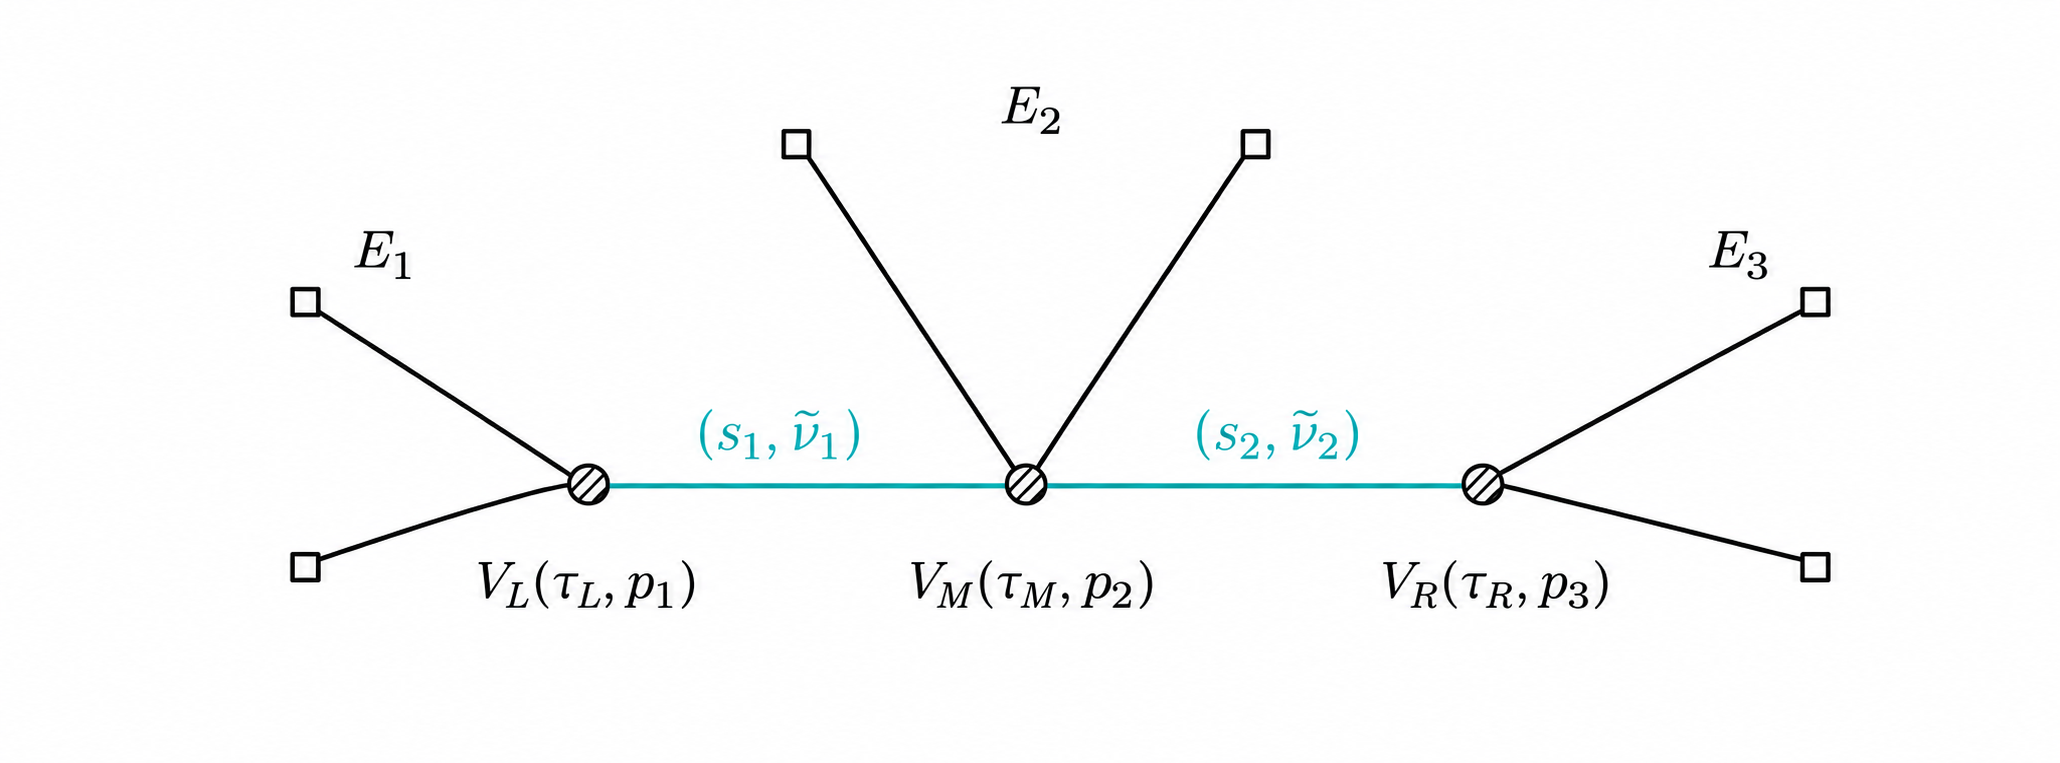
\includegraphics[width=0.92\textwidth]{figures/three_vertex_tree.png}
  \caption{Tree with three vertices and two massive scalar propagators.
  The external energy sums are $E_1,E_2,E_3$. The internal lines carry
  momentum magnitudes $s_1,s_2$ and mass labels
  $\widetilde\nu_1,\widetilde\nu_2$.}
  \label{fig:tree-diagram}
\end{figure}

The vertices $L,M,R$ have conformal times $\tau_L,\tau_M,\tau_R$.
The two internal lines connect $L$ to $M$ and $M$ to $R$, respectively.
Each $E_i$ is the sum of the external momentum magnitudes at vertex $i$.
The internal momentum magnitudes are $s_1,s_2$, and the Hankel orders are
$\nu_1,\nu_2$. For the masses in the principal series used here,
$\nu_i=\ii\widetilde\nu_i$, with real $\widetilde\nu_i$.
Each vertex has a contour sign $\sigma_v=\pm1$.

We first define the endpoint states used to label the master integrals. This
application is evaluated in the \texttt{NuConvention -> "Negative"} option, i.e.\ with
$s_\nu=-1$ in the unified definition of Sec.~\ref{sec:notation}, because the physical mode
functions and the printed formulae of \cite{Chen:2024glu} that we benchmark against are written in
that option:
\begin{equation}
 \begin{aligned}
 h^{(r)}(\nu,0;z)&=z^{-\nu}H^{(r)}_\nu(z),\\
 h^{(r)}(\nu,1;z)&=\partial_z h^{(r)}(\nu,0;z)
                  =-z^{-\nu}H^{(r)}_{\nu+1}(z),
 \qquad r=1,2.
 \end{aligned}
 \label{eq:application-endpoint-states}
\end{equation}
Nothing here is a third convention: the package default is $s_\nu=+1$, with
$h^{(r)}(\nu,0;z)=z^{+\nu}H^{(r)}_\nu(z)$ and
$h^{(r)}(\nu,1;z)=z^{+\nu}H^{(r)}_{\nu-1}(z)$, and the two readings are related by the single
simultaneous replacement $\nu\to-\nu$ of Sec.~\ref{sec:notation}, which must also be applied to the
effective time powers below.
Here $r$ selects the Hankel function and the binary index selects the
undifferentiated or differentiated state. We use the same Hankel order
at both ends of each line; constant factors from the physical mode
normalisation are restored when forming the correlator.
To display the time ordering explicitly, define
\begin{equation}
 \begin{aligned}
 W^>_{\nu;ab}(s;\tau,\tau')
 &=h^{(1)}(\nu,a;-s\tau)h^{(2)}(\nu,b;-s\tau'),\\
 W^<_{\nu;ab}(s;\tau,\tau')
 &=h^{(2)}(\nu,a;-s\tau)h^{(1)}(\nu,b;-s\tau'),
 \qquad a,b\in\{0,1\}.
 \end{aligned}
 \label{eq:application-line-products}
\end{equation}
The corresponding line kernels, with mode prefactors removed, are
\begin{equation}
 \begin{aligned}
 \mathcal G^{++}_{\nu;ab}
 &=\theta(\tau-\tau')W^>_{\nu;ab}
   +\theta(\tau'-\tau)W^<_{\nu;ab},\\
 \mathcal G^{--}_{\nu;ab}
 &=\theta(\tau-\tau')W^<_{\nu;ab}
   +\theta(\tau'-\tau)W^>_{\nu;ab},\\
 \mathcal G^{+-}_{\nu;ab}&=W^<_{\nu;ab},\qquad
 \mathcal G^{-+}_{\nu;ab}=W^>_{\nu;ab}.
 \end{aligned}
 \label{eq:application-line-kernels}
\end{equation}
All kernels in this equation have arguments $(s;\tau,\tau')$.
The binary indices act only on the Hankel factors, not on the step functions.

For $\boldsymbol\sigma=(\sigma_L,\sigma_M,\sigma_R)$, the unpinched master
integrals are
\begin{equation}
 \begin{aligned}
 I^{\boldsymbol\sigma}_{abcd}
 ={}&\int_{-\infty}^{0}d\tau_L\,d\tau_M\,d\tau_R\,
 (-\tau_L)^{\nu_{0L}}(-\tau_M)^{\nu_{0M}}(-\tau_R)^{\nu_{0R}}\\
 &\times e^{\ii(\sigma_LE_1\tau_L+\sigma_ME_2\tau_M+\sigma_RE_3\tau_R)}\\
 &\times\mathcal G^{\sigma_L\sigma_M}_{\nu_1;ab}(s_1;\tau_L,\tau_M)
 \mathcal G^{\sigma_M\sigma_R}_{\nu_2;cd}(s_2;\tau_M,\tau_R).
 \end{aligned}
 \label{eq:tree-indexed-masters}
\end{equation}
Here $a,b,c,d\in\{0,1\}$. Each time integral runs from $-\infty$ to $0$ with the Bunch--Davies
prescription. The four indices refer to the endpoints
$(L_1,M_1,M_2,R_2)$, in that order. Thus the Top vector is
\begin{equation}
 \bm I^{\boldsymbol\sigma}_{\mathrm{Top}}
 =\bigl(I^{\boldsymbol\sigma}_{0000},
        I^{\boldsymbol\sigma}_{0001},\ldots,
        I^{\boldsymbol\sigma}_{1111}\bigr)^{\mathsf T}.
 \label{eq:tree-top-vector}
\end{equation}
It contains $2^4=16$ masters. In particular, Top $0000$ denotes
$I^{\boldsymbol\sigma}_{0000}$, with no endpoint derivatives or additional
integer shifts in the time powers.

The parameters $\nu_{0L},\nu_{0M},\nu_{0R}$ in the integrand are the
effective vertex time powers. If $p_1,p_2,p_3$ are the powers before
absorbing the massive mode prefactors, then
\begin{equation}
 \begin{aligned}
 \nu_{0L}&=p_1+\frac32+\nu_1,\qquad
 \nu_{0R}=p_3+\frac32+\nu_2,\\
 \nu_{0M}&=p_2+3+\nu_1+\nu_2.
 \end{aligned}
 \label{eq:tree-time-power-map}
\end{equation}
The vertex factors $\ii\sigma_v$ and the external and mode normalisations
are not included in \eqref{eq:tree-indexed-masters}; they are restored
when constructing the physical correlator.

In the IBP reduction, derivatives of the functions that impose time ordering generate
contact terms that merge adjacent vertices. These terms define the
LeftPinch, RightPinch and DoublePinch sectors.
Their masters can be labelled $I^{\boldsymbol\sigma,L}_{cd}$,
$I^{\boldsymbol\sigma,R}_{ab}$ and $I^{\boldsymbol\sigma,D}$, respectively.
The left pinch merges $L$ and $M$ and leaves the two indices of line 2;
the right pinch merges $M$ and $R$ and leaves those of line 1.
The double pinch merges all three vertices and leaves no massive line.
When both internal lines join vertices with equal contour signs, the full
hierarchy is
\begin{equation}
  \mathrm{Top}(16)\oplus\mathrm{LeftPinch}(4)\oplus
  \mathrm{RightPinch}(4)\oplus\mathrm{DoublePinch}(1),
  \qquad \dim=25.
  \label{eq:tree-hierarchy}
\end{equation}
For other contour assignments, only the allowed pinched sectors are included.

At real kinematic points, we compute the four assignments
$(+++)$, $(++-)$, $(+-+)$ and $(-++)$.
After restoring the vertex factors and mode normalisations, each
Top $0000$ entry gives one contribution to the physical correlator.
Reversing all three contour signs gives the complex conjugate contribution.
The four computed terms and their conjugates determine
$\mathcal A_{\mathrm{phys}}$.
To match the phase convention above, the application code passes $-E_v$ as \texttt{externalLegEnergy}, uses \texttt{NuConvention -> "Negative"}, and supplies the corresponding pinch normalisations.

We set $p_1=p_2=p_3=0$ and express all energies and momenta in units of $E_2$.
With $q=s_1/E_2$, the scan follows
\begin{equation}
 \begin{aligned}
 (E_1,E_2,E_3,s_1,s_2)
 &=\left(\frac{100q}{99},1,\frac{10}{99},q,\frac{1}{10}\right),
 & (\nu_1,\nu_2)&=(\ii,2\ii),\\
 (\nu_{0L},\nu_{0M},\nu_{0R})
 &=\left(\frac32+\ii,3+3\ii,\frac32+2\ii\right).&&
 \end{aligned}
 \label{eq:tree-slice}
\end{equation}

For an independent analytic check, we use the multivariable
hypergeometric representation of this correlator derived
in ref.~\cite{Xianyu:2023ytd}.
It expresses the signal and background contributions as multiple series
containing Appell $F_2$ functions. Their sum gives the complete physical
correlator. These contributions are not the IBP sectors in
\eqref{eq:tree-hierarchy}.
For this benchmark, DE transport evolves the full master vector for each
contour assignment and then extracts the physical correlator from its
$I^{\boldsymbol\sigma}_{0000}$ entries. The hypergeometric calculation
evaluates the same physical correlator directly at each target point;
it does not separately evaluate all components of the master vectors.
The reported comparison is therefore between physical correlators,
not a componentwise comparison of all masters.
The truncation order is selected by comparing adjacent orders.
The reported hypergeometric time is the sum of the accepted
pointwise evaluation times.

The DE calculation uses 80 decimal digits and local Taylor series truncated at order 80.
An independent transport at order 96 provides an internal stability check.
We compare batches of $N=1$, $10$, $50$ and $100$ target points on the slice in \eqref{eq:tree-slice}.
For $N=1$, $10$ and $50$, transport starts at $q=0.1$ and ends at $q=10^{-4}$.
The single point is the endpoint, corresponding to $x=-\log_{10}q=4$.
The ten points are selected at approximately equal index intervals from the original 50 points, including both endpoints.
The 100 point batch contains 80 points on this path and 20 additional points from $q=0.105$ to $0.2$.
The additional points share the boundary at $q=0.1$ but require transport in the opposite direction.

The hypergeometric times for these four batches are $22.78$, $344.62$, $1040.95$ and $4242.89\,\mathrm{s}$.
The corresponding median DE times are $26.71$, $48.82$, $48.86$ and $57.56\,\mathrm{s}$
(figure~\ref{fig:tree-timing}).
Each DE time includes physical boundary construction, DE generation and the transport call, with the order 96 backend time subtracted.
It includes data preparation and Python invocation.
All four DE batches were measured three times, with the execution order varied between rounds.
We report the median total time and show the full range of the three measurements.
The observed ratios of hypergeometric time to DE time are $7.06$, $21.31$ and $73.71$ for ten, 50 and 100 points, respectively.
The isolated endpoint is slower with DE transport than with the hypergeometric representation.

The average DE time per output point decreases from $26.71\,\mathrm{s}$ to $4.88$, $0.98$ and $0.58\,\mathrm{s}$ across these batches.
Boundary data and transport are shared, rather than recomputed independently for each target.
Points encountered along the path use saved node values or evaluations of an already constructed local series.
In the new tests, each branch used 29 internal nodes for one output point and 33 nodes for ten output points.
Thus, additional outputs did not require a proportional increase in transport work.

Within a convergence disk, a shorter step suppresses higher Taylor terms.
It can therefore permit a lower truncation order at a fixed accuracy.
This is a local property, not a guarantee of lower total cost, since shorter steps can require more segments.

\begin{figure}[H]
  \centering
  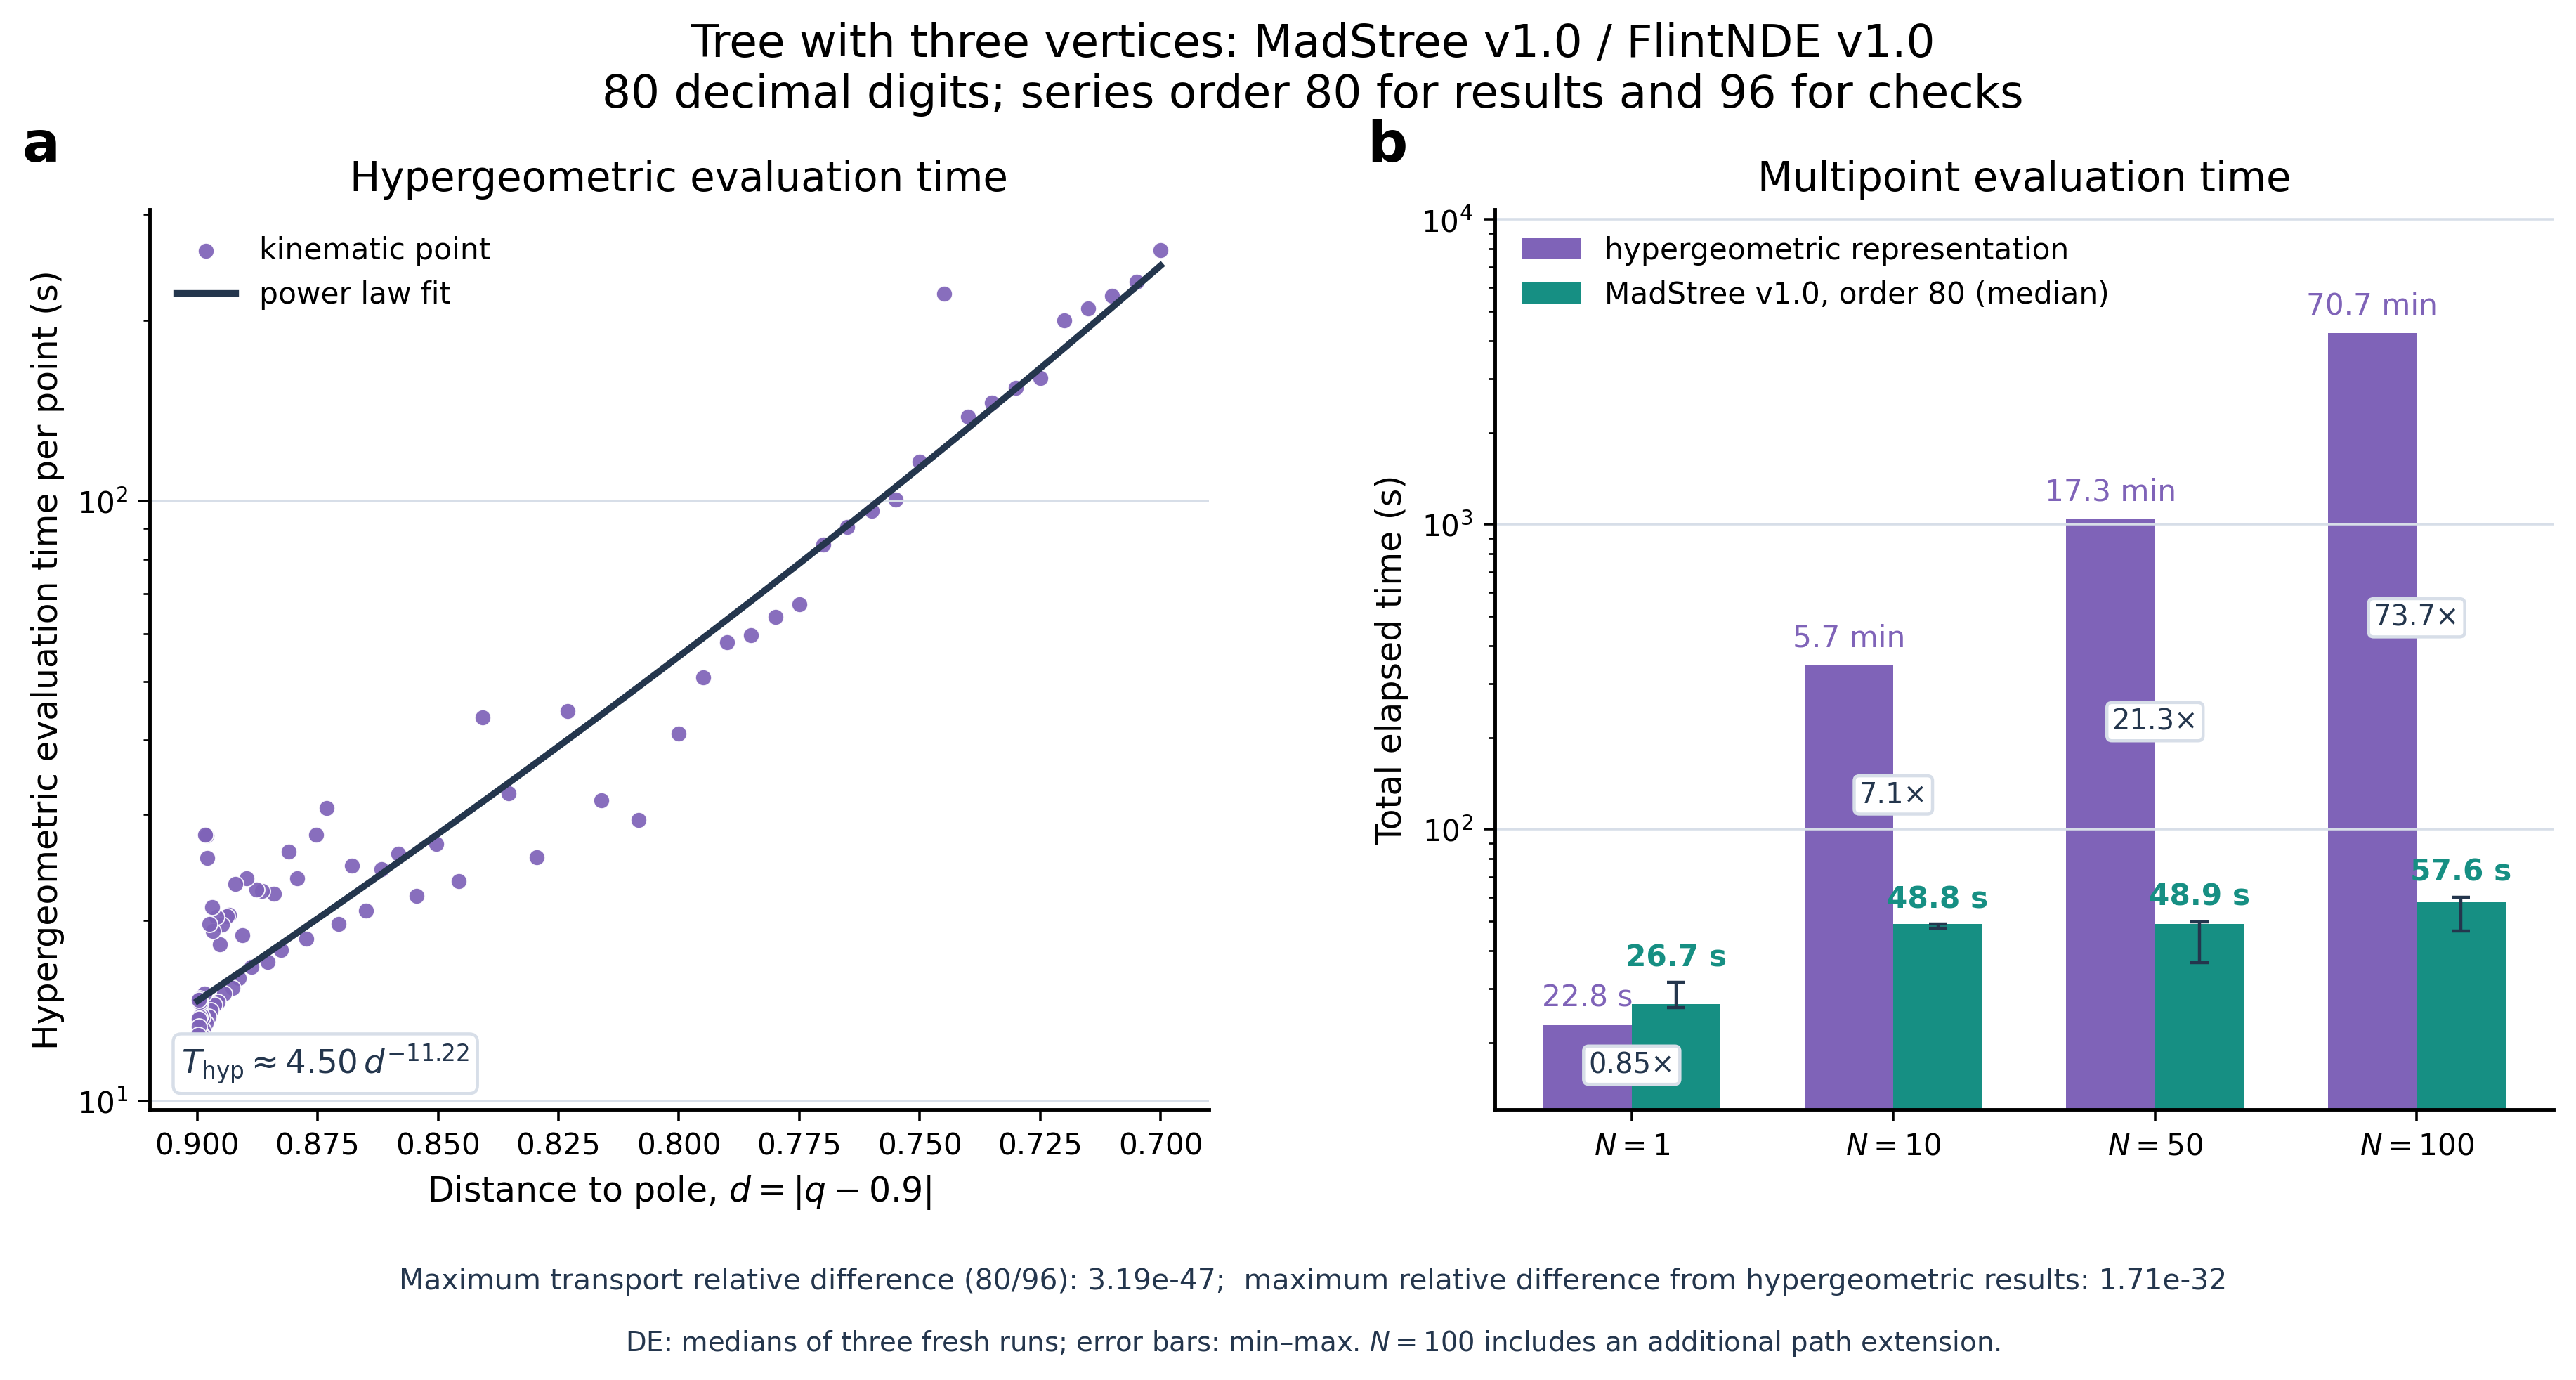
\includegraphics[width=0.99\textwidth]{figures/time.png}
  \caption{Tree benchmark with MadStree v1.0 and FlintNDE v1.0.
  \textbf{a}, Hypergeometric evaluation time at individual kinematic points.
  \textbf{b}, Total evaluation times for $N=1$, $10$, $50$ and $100$ target points.}
  \label{fig:tree-timing}
\end{figure}

The 100 points in figure~\ref{fig:tree-timing}\textbf{a} comprise 80 points with
$q=10^{-x}$ and $x=1+3j/79$ ($j=0,\ldots,79$), uniformly spaced in $x$, and
20 points with $q=0.1+0.005j$ ($j=1,\ldots,20$), uniformly spaced in $q$.
Each hypergeometric time uses the accepted truncation order.
In panel \textbf{b}, the DE bars show medians of three runs, with error bars spanning the minimum and maximum.
The times include boundary construction, DE generation and the transport call. The first three batches share the same start and endpoint; the 100 point batch includes the additional path extension.
Hypergeometric data are newly computed for one and ten points and retained for 50 and 100 points.
The ratio labels give the hypergeometric time divided by the DE time.
The figure footer reports the largest relative differences between transport orders and from the hypergeometric results across all four batches.

Across the scan of 100 points, the largest relative difference from the
hypergeometric result is $1.712\times10^{-32}$.
The comparison of transport orders 80 and 96 gives a maximum relative difference
of $1.308\times10^{-50}$.
At $x=4$, the physical correlator is
\begin{equation}
  \mathcal A_{\mathrm{phys}}(4)=9.87033514798954\times10^{-9},
\end{equation}
with a relative difference of $4.21\times10^{-36}$ from the hypergeometric result.

On the same kinematic configuration, the direct Appell $F_2$ representation
requires $q<0.89$.
The point $q=0.8905$ lies outside this domain, whereas the nearest positive
pole of the DE connection is at $q=0.9$.
To reach $q=1$, we continue the chosen analytic branch along
\begin{equation}
  0.1\to0.86\to0.86+0.04\ii\to0.93+0.04\ii\to0.93\to1.
  \label{eq:tree-contour}
\end{equation}
This contour avoids the pole through the upper half of the complex plane.
The continuation records 81 points.
The calculation at order 80 takes $35.08$~s, or $45.76$~s when the reference calculation at order 96 is included.
The maximum relative difference between orders 80 and 96 is $1.802\times10^{-44}$.
Within the overlap region, the maximum relative difference from the
hypergeometric result is $1.712\times10^{-32}$.
The DE method thus evaluates the selected analytic branch beyond the
domain of the direct series representation.

\begin{figure}[H]
  \centering
  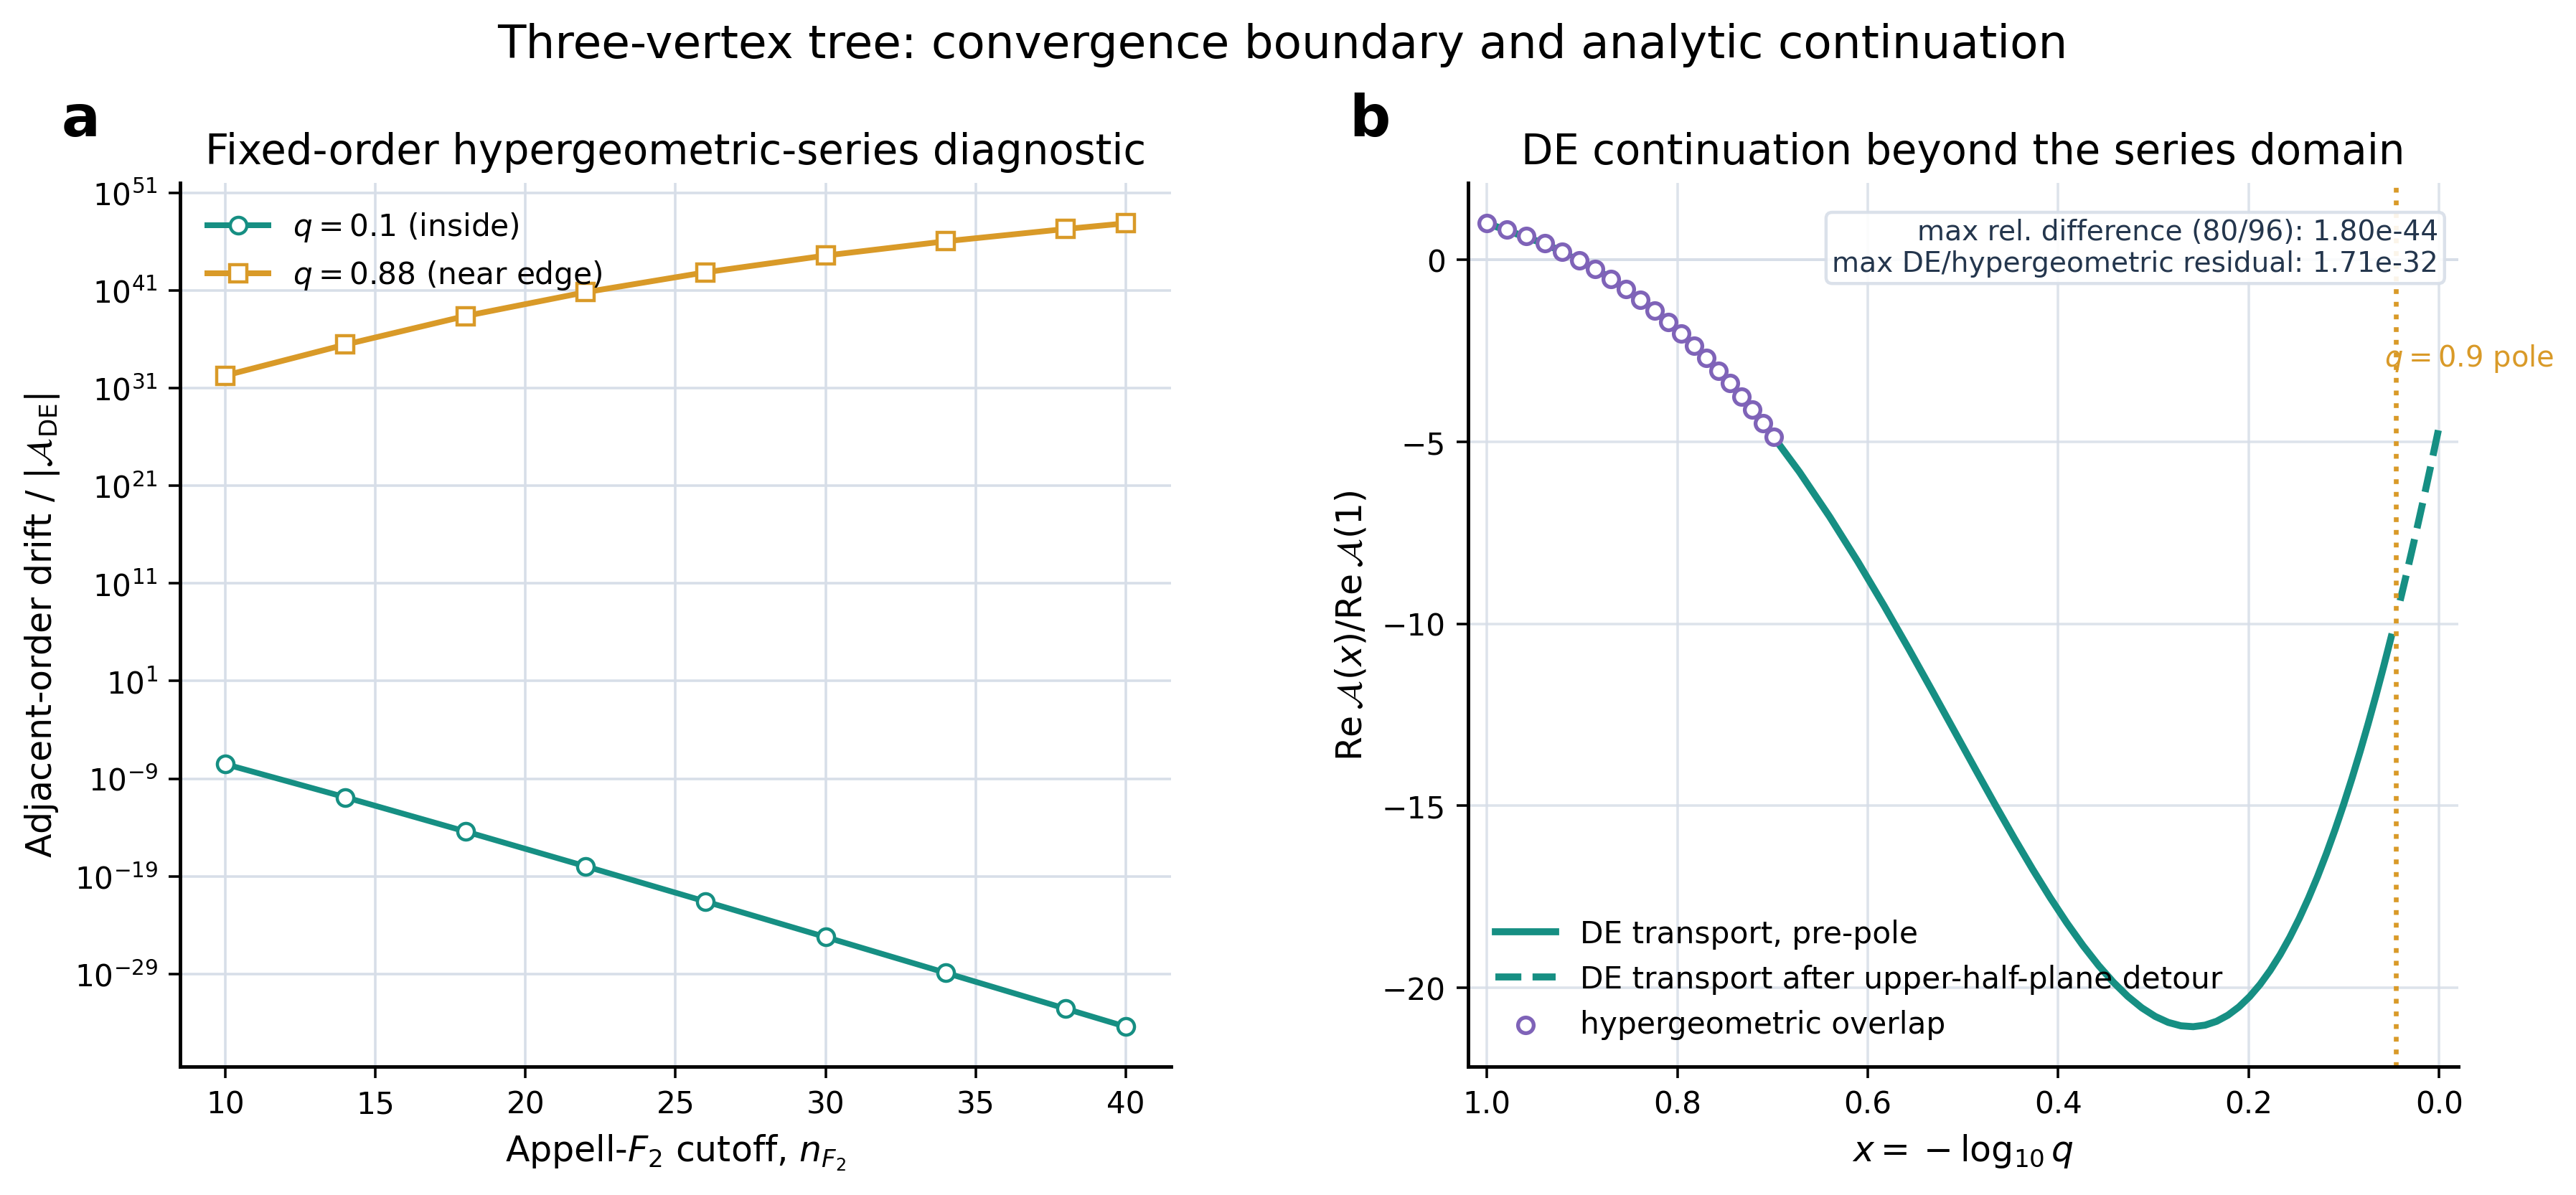
\includegraphics[width=0.99\textwidth]{figures/domain1.png}
  \caption{Analytic continuation with MadStree v1.0.
  \textbf{a}, Dependence of the hypergeometric partial sums on the truncation
  order near the direct convergence boundary.
  \textbf{b}, DE continuation at order 80 along the contour
  in \eqref{eq:tree-contour}.}
  \label{fig:tree-continuation}
\end{figure}

\paragraph{Bubble time kernel at fixed loop momentum}

The second example has two time vertices joined by two massive propagators
(figure~\ref{fig:bubble-diagram}).
We evaluate the integrals over the two vertex times while holding the internal
momenta fixed. We do not integrate over the spatial loop momentum.
\begin{figure}[H]
  \centering
  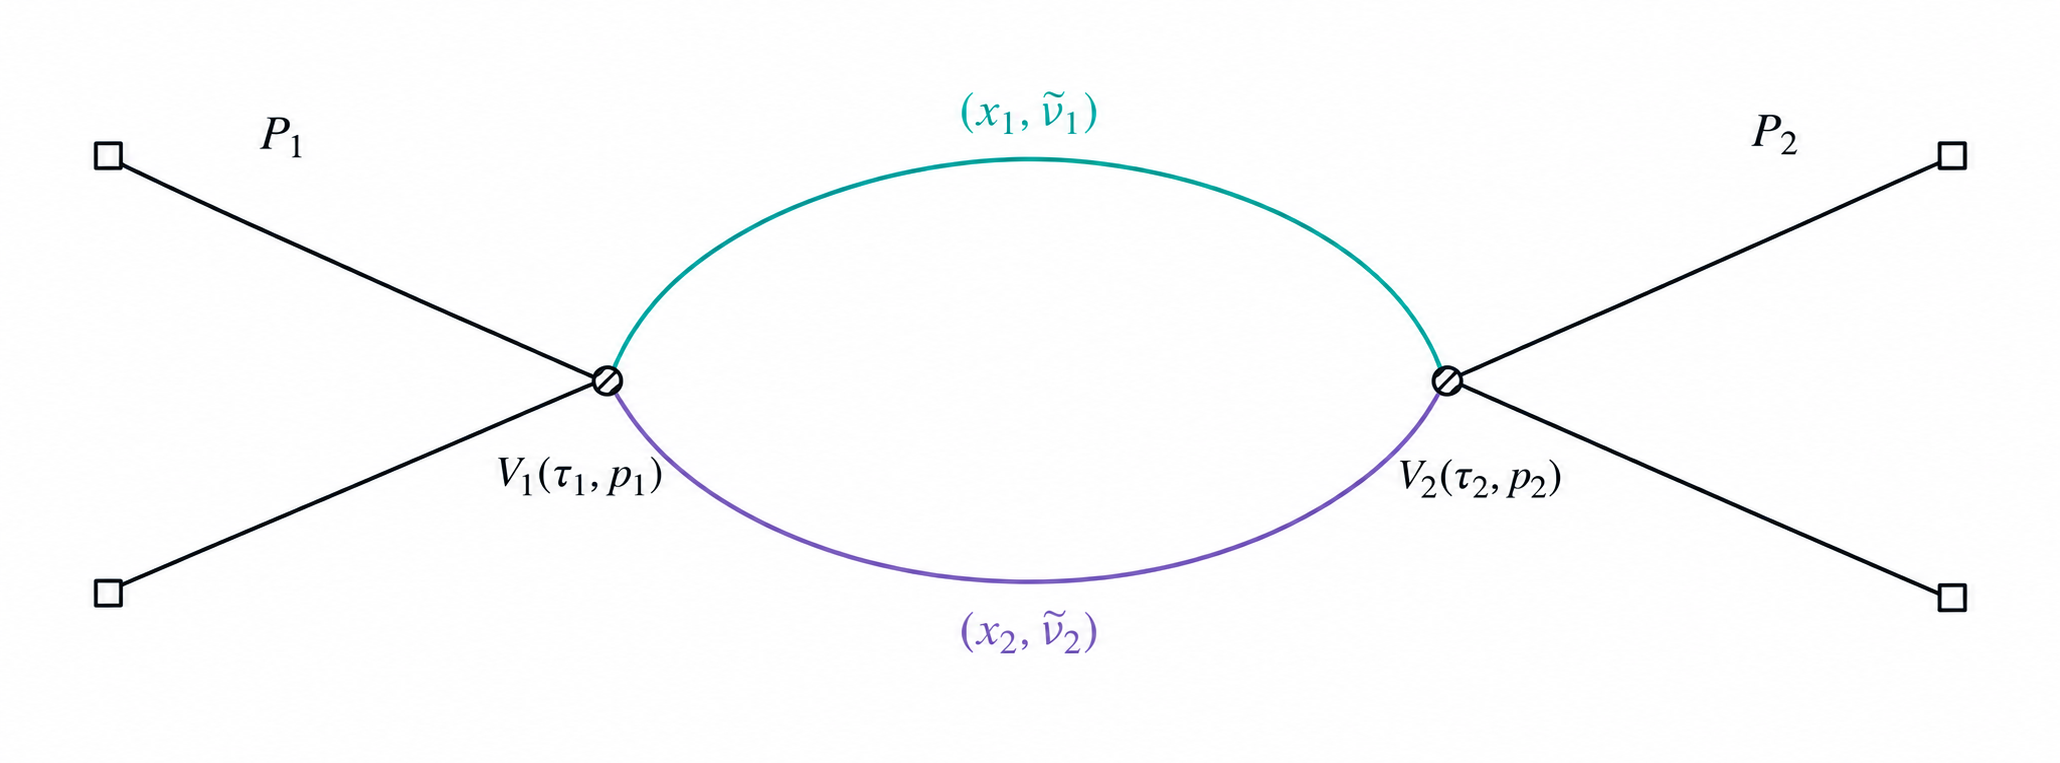
\includegraphics[width=0.90\textwidth]{figures/bubble1.png}
  \caption{Bubble time kernel with external energy sums $P_1,P_2$ and
  fixed internal momentum magnitudes $x_1,x_2$.}
  \label{fig:bubble-diagram}
\end{figure}

Let $\tau_1,\tau_2$ be the vertex times, $P_1,P_2$ the external energy sums,
and $x_1,x_2$ the internal momentum magnitudes.
The Hankel orders of the two internal lines are $\nu_{B1},\nu_{B2}$.
Using the line kernels in \eqref{eq:application-line-kernels}, the Top masters are
\begin{equation}
 \begin{aligned}
 J^{\sigma_1\sigma_2}_{abcd}
 ={}&\int_{-\infty}^{0}d\tau_1\,d\tau_2\,
 (-\tau_1)^{p_1}(-\tau_2)^{p_2}
 e^{\ii(\sigma_1P_1\tau_1+\sigma_2P_2\tau_2)}\\
 &\times\mathcal G^{\sigma_1\sigma_2}_{\nu_{B1};ab}(x_1;\tau_1,\tau_2)
 \mathcal G^{\sigma_1\sigma_2}_{\nu_{B2};cd}(x_2;\tau_1,\tau_2).
 \end{aligned}
 \label{eq:bubble-indexed-masters}
\end{equation}
Here $a,b,c,d\in\{0,1\}$. The indices $a,b$ label the two endpoints of line 1 at vertices 1 and 2;
$c,d$ label those of line 2 in the same vertex order.
Here $p_1,p_2$ are the effective time powers after absorbing the mode
prefactors, unlike the bare powers used in \eqref{eq:tree-time-power-map}.
The contour signs are $\sigma_1,\sigma_2=\pm1$.
We denote positive and negative signs by $p$ and $m$, respectively;
these labels are unrelated to the time powers $p_1,p_2$.
The four contour assignments are $pp$, $pm$, $mp$ and $mm$.
In MadStree v1.0, assignments with equal contour signs have 22 masters after the
exact state projection. Assignments with opposite contour signs have only the Top sector, with 16 masters.
For each assignment, the projection onto the Top sector is
$\bm J_{\sigma_1\sigma_2}
=(J^{\sigma_1\sigma_2}_{0000},J^{\sigma_1\sigma_2}_{0001},\ldots,
J^{\sigma_1\sigma_2}_{1111})^{\mathsf T}$.
The vertex factors $(\ii\sigma_1)(\ii\sigma_2)$ give
\begin{equation}
  \bm K_{\mathrm{SK}}=-\bm J_{pp}+\bm J_{pm}+\bm J_{mp}-\bm J_{mm}.
  \label{eq:bubble-sk}
\end{equation}
We use $k_s=x_1$ as the momentum unit and vary the dimensionless energy
$\rho=P_1/k_s=P_2/k_s$. The parameter values in
\eqref{eq:bubble-indexed-masters} are
\begin{equation}
 \begin{aligned}
 (k_s,x_1,x_2)&=(1,1,\sqrt2),\qquad P_1=P_2=\rho,\\
 (\nu_{B1},\nu_{B2})&=(\ii/4,\ii/4),\qquad
 p_1=p_2=1+\ii/2.
 \end{aligned}
 \label{eq:bubble-parameters}
\end{equation}
The normalised Top $0000$ component is
\begin{equation}
  \widehat{\mathcal F}_{\ii/4}(\rho)
  =\frac{[\bm K_{\mathrm{SK}}(\rho)]_{0000}}
  {[\bm K_{\mathrm{SK}}(10)]_{0000}}.
  \label{eq:bubble-normalised}
\end{equation}
The four zeros select the undifferentiated states at the four endpoints of the massive lines.

The scan contains 201 points over $2.8\leq\rho\leq10$.
Calculations use decimal arithmetic with 80 digits. The transport orders are
80 and 96, and the boundary series orders are 17 and 15.
The calculation time excluding reference transport at order 96 is $678.20$~s.
It includes all four contour assignments, DE construction and both
boundary calculations.
The reference transport takes $5.24$~s, and the total recorded time is
$683.43$~s.
The average cost for the scan, including setup, is $3.37$~s per point.
This average is not the cost of a calculation at a single point.

The maximum relative difference between boundary orders 17 and 15 is
$4.740\times10^{-24}$.
The maximum relative difference between transport orders 80 and 96 is
$1.025\times10^{-50}$.
These tests assess boundary and transport stability separately; the
comparison of transport orders alone is not a bound on the total error.
The largest relative difference from the independent scan is
$3.70\times10^{-14}$.

\begin{figure}[H]
  \centering
  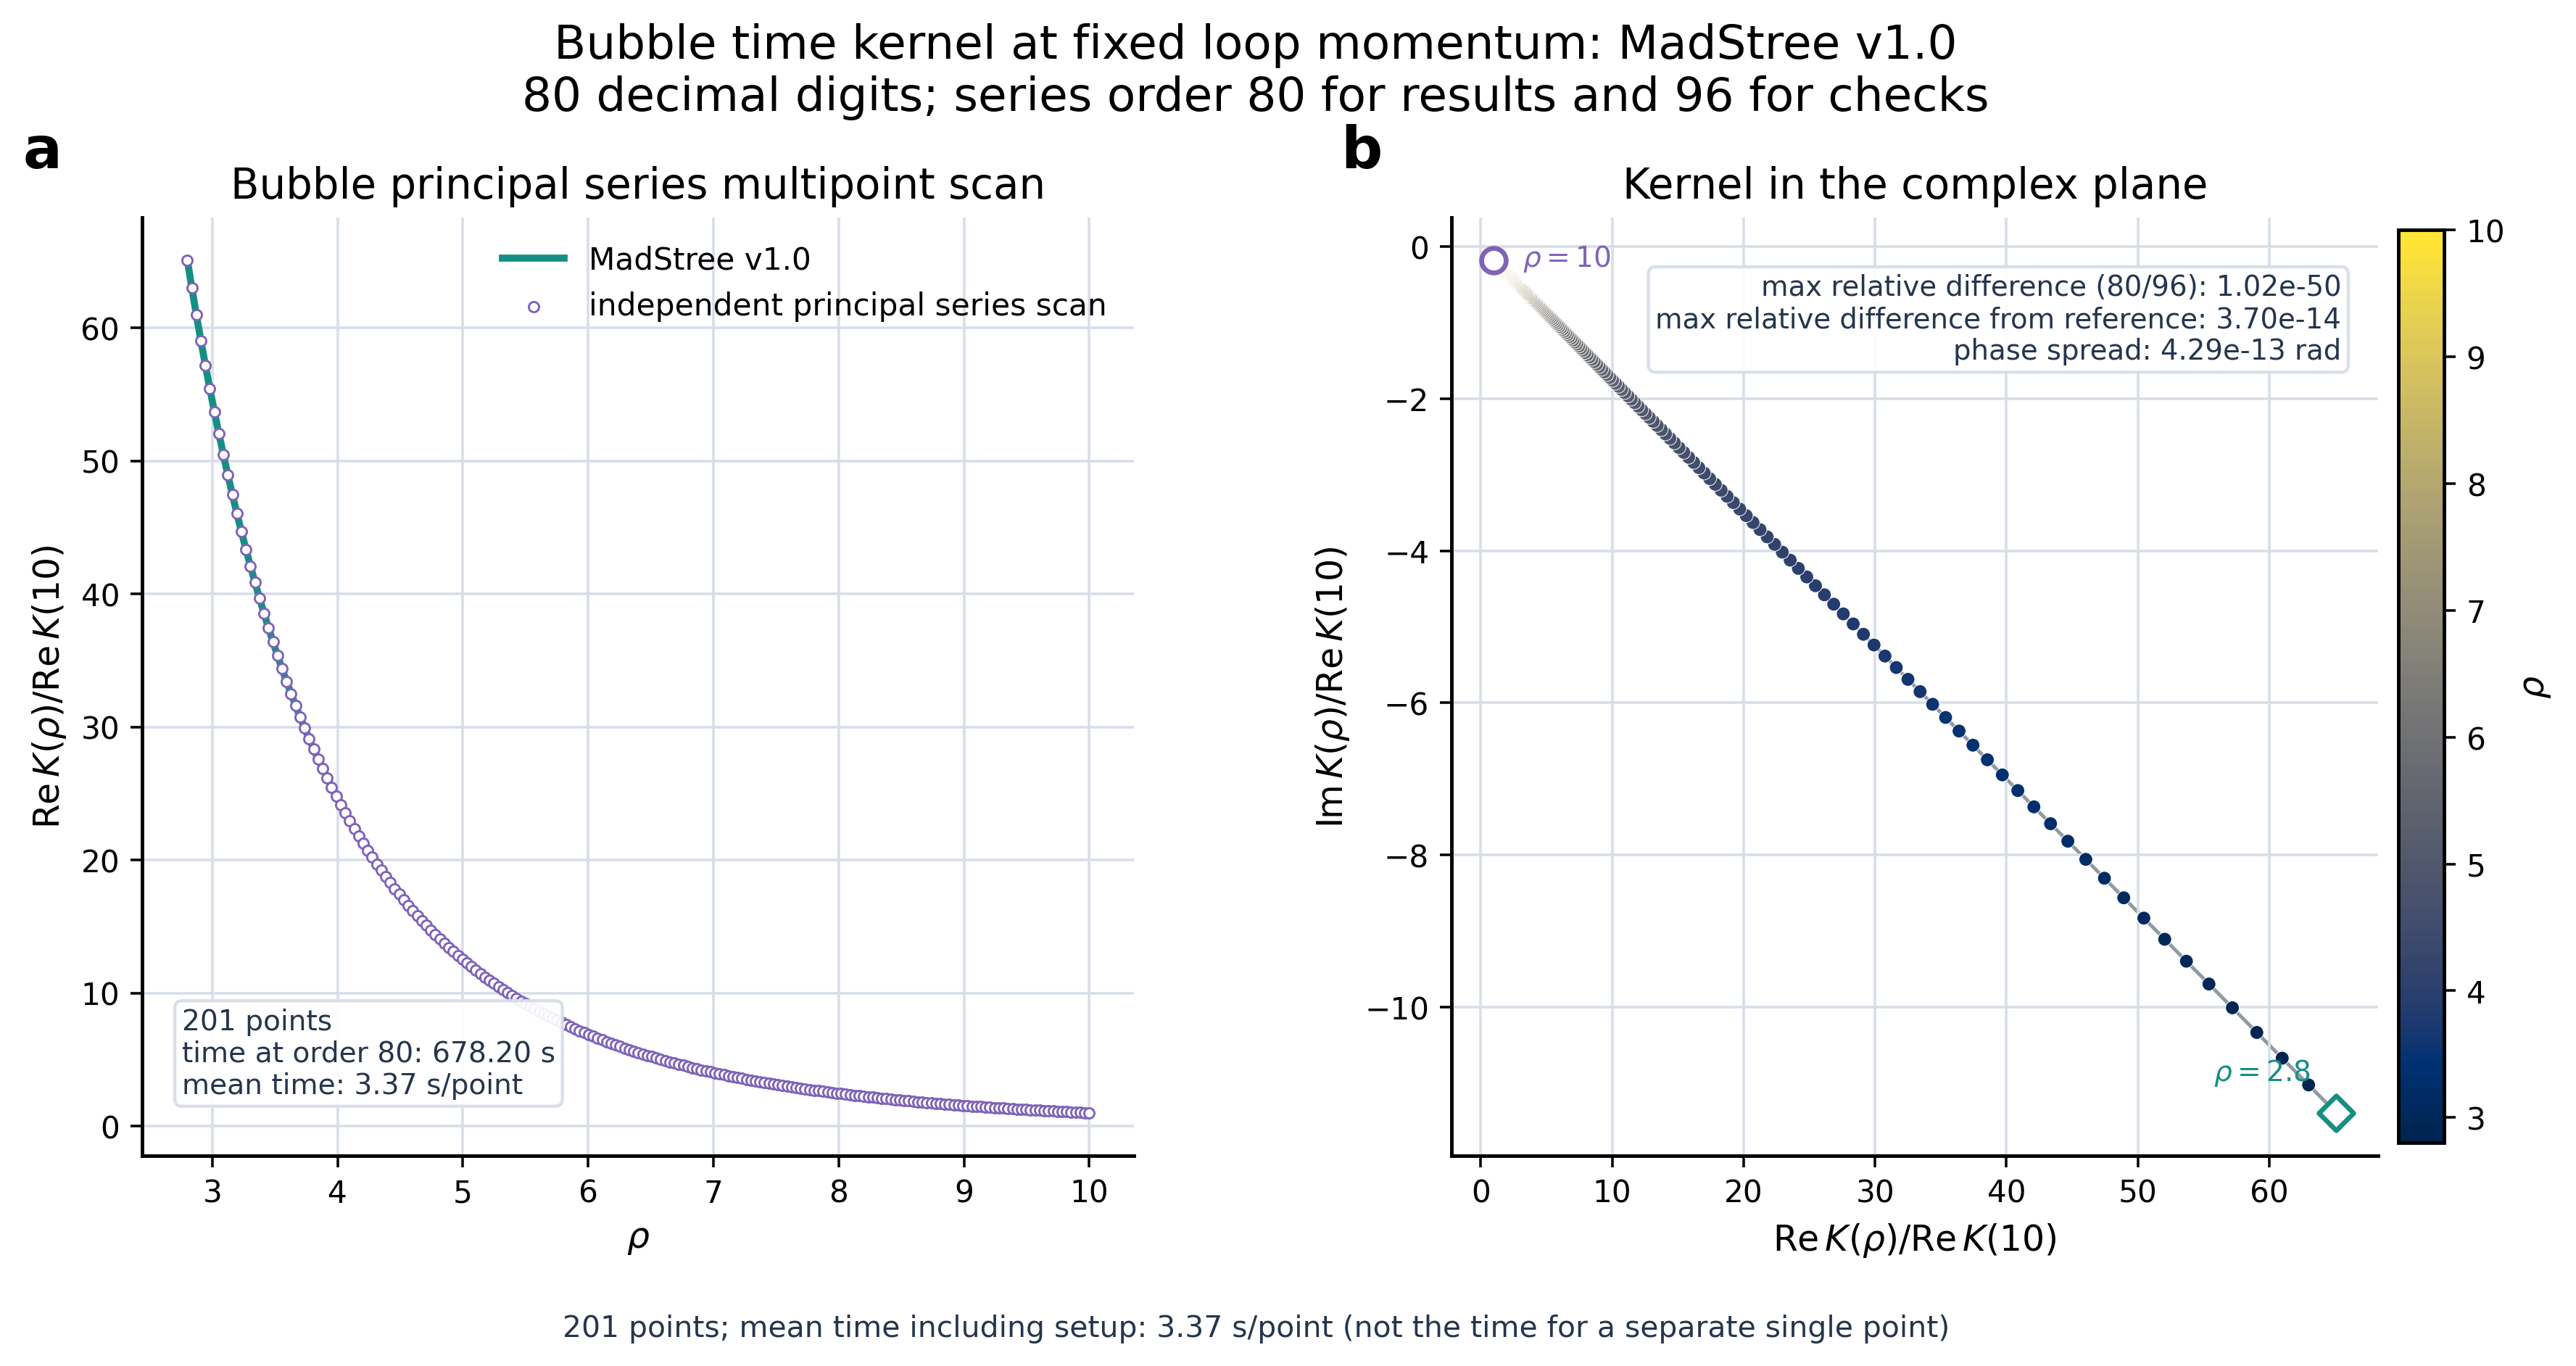
\includegraphics[width=0.99\textwidth]{figures/bubble2.png}
  \caption{Bubble time kernel evaluated with MadStree v1.0.
  \textbf{a}, The normalised kernel and the independent reference.
  \textbf{b}, The kernel in the complex plane, with colour indicating $\rho$.}
  \label{fig:bubble-scan}
\end{figure}

Both panels in figure~\ref{fig:bubble-scan} use the same 201 points.
The nearly radial distribution in panel \textbf{b} indicates an approximately constant phase.
The maximum relative difference between transport orders 80 and 96 is $1.025\times10^{-50}$.
The average calculation time, including setup, is $3.37$~s per point; this is the batch average, not an isolated point timing.

The tree example illustrates two uses of DE transport: efficient multipoint
evaluation and continuation beyond the convergence domain of a direct series.
The bubble example applies the same framework for time integrals to a graph
containing a loop at fixed internal momenta.




\section{Summary and outlook}
\label{sec:summary}



\appendix

\section{Common-theta bundles and the odd-subset expansion}
\label{app:theta}

\paragraph{Bundles and their theta argument.}
Fix a sector $s$ and write $\operatorname{comp}_s(v)$ for the current component that contains the
vertex $v$; a component is a maximal set of vertices already merged by contacts, and a lone vertex
is one component. An uncontracted full line $e=(u_e,v_e)$ carries the theta
$\theta(\tau_{u_e}-\tau_{v_e})$ of its two component times, so two lines $e,e'$ carry the
\emph{same} theta if and only if their component pairs coincide as ordered pairs,
\begin{equation}
  \begin{aligned}
  \bigl(\operatorname{comp}_s(u_e),\operatorname{comp}_s(v_e)\bigr)
  &=\bigl(\operatorname{comp}_s(u_{e'}),\operatorname{comp}_s(v_{e'})\bigr)=(U,V),\\
  \text{so}\quad \Delta_e&=\Delta_{e'}\equiv\Delta=\tau_U-\tau_V .
  \end{aligned}
  \label{eq:bundle-criterion}
\end{equation}
A maximal set of lines with this property is the common-theta bundle $\cB$ of the pair $(U,V)$, with
$|\cB|=n\ge2$; the case $n=1$ is an ordinary single-edge contact and is contained in
Sec.~\ref{sec:remaining}. Lines whose theta arguments differ belong to different bundles, and the
bundles are independent because their $\Delta$'s are independent variables: the contact events are
therefore performed bundle by bundle, never across bundles. The vertex exponentials of Block (i) are
theta-free and take no part in this bookkeeping, so only the endpoint factors of
\eqref{eq:sk-propagators} enter the steps below.

\paragraph{Step 1: multiplying the thetas out.}
For each edge of one bundle, write the SK pair of endpoint products as in \eqref{eq:sk-propagators},
$\alpha_e$ for the coefficient of $\theta(\Delta)$ and $\beta_e$ for that of $\theta(-\Delta)$. At
the level of the $h$ blocks the two are the two orderings of the Hankel branches,
\begin{equation}
  \alpha_e = h^{(1)}_{u_e}\,h^{(2)}_{v_e},
  \qquad
  \beta_e = h^{(2)}_{u_e}\,h^{(1)}_{v_e},
  \label{eq:bundle-alphabeta}
\end{equation}
where the orders, states and arguments are those of \eqref{eq:h-definition}; $G^{--}$ interchanges
the two names, and this is the only place the sign $\sigma_e$ of the bundle enters. The product of
the bundle is a product of $n$ binomials in the two functions $\theta(\Delta)$ and
$\theta(-\Delta)$. Expanding naively gives $2^n$ terms, but inside one bundle $\theta(\Delta)$ is
the \emph{same} function for every factor, so idempotency $\theta(\Delta)^2=\theta(\Delta)$ makes
all powers of one argument collapse to that argument, and orthogonality
$\theta(\Delta)\theta(-\Delta)=0$ annihilates every term containing both arguments. Exactly the two
terms of \eqref{eq:bundle-two-terms} survive. The factor $2^n$ thus never appears within a bundle:
it counts the events of $n$ lines with pairwise different theta arguments, which is the case of $n$
different bundles, and those are enumerated bundle by bundle.

\paragraph{Step 2: one theta gives one delta.}
Differentiating the two-term form with respect to the single variable $\Delta$ gives
\begin{equation}
  \partial_\Delta\!\left[\theta(\Delta)\prod_{e\in\cB}\alpha_e
  +\theta(-\Delta)\prod_{e\in\cB}\beta_e\right]
  =\delta(\Delta)\left(\prod_{e\in\cB}\alpha_e-\prod_{e\in\cB}\beta_e\right),
  \label{eq:bundle-delta}
\end{equation}
because $\partial_\Delta\theta(\Delta)=\delta(\Delta)$ and
$\partial_\Delta\theta(-\Delta)=-\delta(\Delta)$. Three consequences are worth stating explicitly.
First, the bundle produces \emph{one} distribution, not $n$ of them: the whole contact information
of the bundle is concentrated in the single coefficient
$\prod_e\alpha_e-\prod_e\beta_e$, which is antisymmetric under
$\alpha\leftrightarrow\beta$. Second, that one $\delta(\Delta)$ forces the two component times to
coincide \emph{once}, so the components $U$ and $V$ merge once, independently of how many factors
$\mathsf d_e$ a term of the coefficient contains; this is what fixes the merge count in
\eqref{eq:base-power}. Third, for $G^{--}$ the interchange of $\alpha$ and $\beta$ turns
\eqref{eq:bundle-delta} into its negative, which reproduces the single sign $\sigma_e$ of
\eqref{eq:contact-weight} for a whole bundle.

\paragraph{Step 3: telescoping the antisymmetric difference.}
Order the edges of the bundle as $1,\dots,n$ and abbreviate $\alpha_e=A_e$, $\beta_e=B_e$. Inserting
and subtracting successive partial products gives the telescoping identity
\begin{equation}
\begin{split}
  \prod_{e=1}^{n}A_e-\prod_{e=1}^{n}B_e
  &=\sum_{k=1}^{n}\left(\prod_{e\leq k}A_e\prod_{e>k}B_e
  -\prod_{e< k}A_e\prod_{e\geq k}B_e\right)\\
  &=\sum_{k=1}^{n}D_k\prod_{e<k}A_e\prod_{e>k}B_e ,
\end{split}
  \label{eq:bundle-telescope}
\end{equation}
whose intermediate sum collapses because the $k$-th second summand and the $(k{+}1)$-th first
summand are identical, while the first summand of $k=1$ and the last summand of $k=n$ supply the two
products of \eqref{eq:bundle-delta}. Each term of \eqref{eq:bundle-telescope} contains exactly one
difference factor $D_e=A_e-B_e$.

\paragraph{Step 4: collecting by subsets and the parity.}
Introduce, as in \eqref{eq:bundle-odd-subsets}, the difference and the mean of the two endpoint
products, $\mathsf d_e=D_e=A_e-B_e$ and $\mathsf m_e=(A_e+B_e)/2$, equivalently
$A_e=\mathsf m_e+\mathsf d_e/2$ and $B_e=\mathsf m_e-\mathsf d_e/2$, and expand the spectators of
\eqref{eq:bundle-telescope} in this basis. In the $k$-th term the edge $k$ supplies the explicit
$\mathsf d_k$; an edge $e\in S$ with $e<k$ contributes $+\mathsf d_e/2$, an edge $e\in S$ with $e>k$
contributes $-\mathsf d_e/2$, and every edge outside $S$ contributes $\mathsf m_e$. So the
coefficient of the monomial $\prod_{e\in S}\mathsf d_e\prod_{e\notin S}\mathsf m_e$ is
\begin{equation}
  c_S = 2^{1-|S|}\sum_{k\in S}(-1)^{\#\{e\in S:\,e>k\}} .
  \label{eq:bundle-coefficient}
\end{equation}
Writing $S=\{i_1<\dots<i_m\}$ with $m=|S|$, the exponent for $k=i_j$ is $m-j$, hence
\begin{equation}
  \sum_{j=1}^{m}(-1)^{m-j}=\sum_{r=0}^{m-1}(-1)^{r}
  =\begin{cases}1,&m\ \text{odd},\\ 0,&m\ \text{even},\end{cases}
  \qquad
  c_S=\bigl(1-(-1)^{|S|}\bigr)2^{-|S|},
  \label{eq:bundle-parity}
\end{equation}
which is \eqref{eq:bundle-odd-subsets}: only odd subsets survive, each with the pure numerical
weight $2^{1-|S|}$. The empty set cannot occur, since every telescoping term carries at least the
explicit $\mathsf d_k$, in agreement with $c_\varnothing=0$. The same parity follows from symmetry
without any enumeration: the left-hand side of \eqref{eq:bundle-telescope} changes sign under
$\alpha\leftrightarrow\beta$, in which $\mathsf d_e$ is odd and $\mathsf m_e$ even, so a monomial
with an even number of $\mathsf d$ factors must cancel; the explicit computation
\eqref{eq:bundle-coefficient} only fixes the remaining coefficients.

\paragraph{Events, weights and the bookkeeping.}
Each non-empty odd subset $S$ of one bundle is one simultaneous contact event. Its injection matrix
$C^{(v,1)}_{st}$ of \eqref{eq:contact-injection} is the tensor product of the local contact
selectors of the edges in $S$ --- $|1\rangle_e$ on a massless shared slot, the complementary-bit
selector of \eqref{eq:R-two-vertex} on a pair of massive endpoints --- multiplied by $2^{1-|S|}$ and
by the spectator factors $\mathsf m_e$ of the unselected bundle edges, then embedded in the global
bit order with all spectator bits of other edges preserved. The collected form
\eqref{eq:bundle-odd-subsets}, not the term-by-term form \eqref{eq:bundle-telescope}, is what the
program enumerates: the $k$-th telescoping term stands for ``contract only the $k$-th line,'' but
after the spectators are expanded the same subset $S$ is reached from several $k$, so an
enumeration over $k$ would generate the same sector transition more than once. After collecting,
each event appears exactly once with a numerical weight, and the deduplication key of the reduction
is the triple (parent sector, child sector, set of selected line identifiers), which is finite
because every event strictly reduces the number of current components.

\paragraph{Child base power and coincident unselected edges.}
For a component $C$ produced by such events the base power is \eqref{eq:base-power},
$A_{C,s}=\sum_{v\in C}\nu_{0,v}+\sum_{e\in E_s(C)}r_e+|C|-1$. The three terms have three different
origins and should not be conflated: the vertex powers add because the merged integrand is a
product, each contracted edge adds its own raw contact power $r_e$ because the corresponding
$\delta$ brings one factor $(-\tau)^{r_e}$, and the last term counts \emph{merges of components},
which is $|C|-1$ for any component of $|C|$ vertices and does not grow with the number of bundle
edges contracted at once. Since \eqref{eq:base-power} depends only on the final component and on
the contracted set, and not on the order or the clustering of the events, different legal event
sequences that reach the same sector give the same child base power; the reduction is confluent at
the level of the powers.

An unselected edge whose two ends fall into one component after a bundle event must also be reduced
at equal times. For a massless full edge the shared slot then contributes only its symmetric state,
because the two Wightman combinations coincide at coincident times, so the odd shared state of the
edge gives zero; for a massive full edge the two single-derivative endpoint states become
identified, $10\sim01$, which is the equal-time canonical quotient. Both cases are implemented the
same way: the matrices are first built in the raw binary space of all endpoint and shared slots and
then retracted to the true sector masters by the constant maps of
\eqref{eq:SP-massless}, $P_s\,M^{\rm raw}\,S_s$, so the equal-time quotients require no further
computation and no dense inversion.

\paragraph{Relation to the single-contact case.}
For $|\cB|=1$ the two-term form \eqref{eq:bundle-two-terms} reduces to the ordinary SK pair of one
line, \eqref{eq:bundle-telescope} to the single difference $\mathsf d_e$, and $c_{\{e\}}=1$, so the
bundle machinery reproduces exactly the single-edge contacts of Sec.~\ref{sec:remaining} and of
\cite{Chen:2023iix}, where every contact is attached to one full line. The new ingredients are the
weight $2^{1-|S|}$, the parity selection, and the identification of the merge count with $|C|-1$
rather than with the number of contracted edges.



\bibliographystyle{JHEP}
\bibliography{references}

\end{document}
